% ----------- Cover Master Thesis Faculty of Sciences ---------------
% This document should be compiled with pdflatex. If you want to use
% latex to compile to dvi/ps, you have to convert the images to (e)ps
%                           -- December 2012
% -------------------------------------------------------------------
\RequirePackage{fix-cm}
\documentclass[12pt,a4paper,oneside]{book}
%
% ------------------------- Load packages ---------------------------
% You can eventually add these while you load other packages
% in case you want to integrate the titlepage with the rest of your thesis
% -------------------------------------------------------------------
\usepackage{graphicx,xcolor,textpos}
%\usepackage{subfigure}
%\usepackage[spanish,es-nodecimaldot]{babel}% for spanish, decimal="."
\usepackage[utf8]{inputenc}					% for spanish
%\usepackage[top=3cm, bottom=2.54cm, left=3cm, right=2.54cm]{geometry} % margins
\usepackage{setspace} 						% flexible spacing
%\setlength{\parskip}{2.5mm} 			    % paragraph space
\usepackage[square,numbers]{natbib} 						% Bibtex bibliography
%\usepackage[style=apa]{biblatex}			% Biber bibliography
\usepackage{amsfonts}						% mathematical formulas
\usepackage{amsmath}
\usepackage{amssymb}
\usepackage{stackengine}
\usepackage[hidelinks]{hyperref}       		% hyperlinks
\usepackage{url} 							% url typesetting
\usepackage{enumerate} 						% numbered lines
\usepackage{cases} 							% numbered cases equations
\usepackage{color, soul}					% highlight text
\usepackage{listings} 						% to insert R code easily
\usepackage{float}							% to avoid figures to float
\lstset{
%	language=R, 						% to set the style of the code
	basicstyle=\small\ttfamily,
	stringstyle=\color{blue},
%	otherkeywords={0,1,2,3,4,5,6,7,8,9},
%	morekeywords={TRUE,FALSE},
%	deletekeywords={data,frame,length,as,character,R},
	keywordstyle=\color{black},
	commentstyle=\color{blue},
}
%
%
%\addbibresource{bibliography.bib}			% Biber bibliography
%
% ------------------------ Page settings -----------------------------
% If you change these, the cover layout will also change.  In that
% case you have to adjust the latter manually.
% --------------------------------------------------------------------
%
\topmargin -10mm
\textwidth 160truemm
\textheight 240truemm
\oddsidemargin 0mm
\evensidemargin 0mm
%
% ---------------------- textpos settings ----------------------------
% Some additional settings for the cover
% --------------------------------------------------------------------
%
\definecolor{green}{RGB}{172,196,0}
\definecolor{bluetitle}{RGB}{29,141,176}
\definecolor{blueaff}{RGB}{0,0,128}
\definecolor{blueline}{RGB}{82,189,236}
\setlength{\TPHorizModule}{1mm}
\setlength{\TPVertModule}{1mm}
%
\begin{document}
%
% ----------------------- Cover --------------------------------------
% Please fill in:
% - The title and subtitle (if applicable)
%         to include a formula in the title or subtitle
%         use  \form{$...$}
% - Your name
% - Your (co)supervisor, mentor (if applicable)
% - Your master
% - The academic year
% --------------------------------------------------------------------
\graphicspath{{./images/main/}} 	          % relative path for images
%
\thispagestyle{empty}
\newcommand{\form}[1]{\scalebox{1.087}{\boldmath{#1}}}
\sffamily
%
\begin{textblock}{191}(-24,-11)
\colorbox{green}{\hspace{139mm}\ \parbox[c][18truemm]{52mm}{\textcolor{white}{FACULTY OF SCIENCE}}}
\end{textblock}
%
\begin{textblock}{70}(-18,-19)
\textblockcolour{}

\includegraphics[height=19.8truemm]{LogoKULeuven}
\end{textblock}
%
\begin{textblock}{160}(-6,63)
\textblockcolour{}
\vspace{-\parskip}
\flushleft
\fontsize{40}{42}\selectfont \textcolor{bluetitle}{Generalized Linear Latent and Mixed Model:}\\[1.5mm]
\fontsize{20}{22}\selectfont method, bayesian estimation, advantages, and applications to educational data. \\
\end{textblock}
%
\begin{textblock}{160}(8,153)
\textblockcolour{}
\vspace{-\parskip}
\flushright
\fontsize{14}{16}\selectfont \textbf{Jose Manuel Rivera Espejo}
\end{textblock}
%
\begin{textblock}{70}(-6,191)
\textblockcolour{}
\vspace{-\parskip}
\flushleft
Supervisor: Prof. Geert Molenbegrhs \\[-2pt]
\textcolor{blueaff}{ Leuven Biostatistics and Statistical Bioinformatics Centre (L-BioStat) }\\[5pt]
Co-supervisor: Prof. Wim Van den Noortgate \\[-2pt]
\textcolor{blueaff}{ Faculty of Psychology and Educational Sciences }\\[5pt]
\end{textblock}
%
\begin{textblock}{160}(8,191)
\textblockcolour{}
\vspace{-\parskip}
\flushright
Thesis presented in fulfillment of\\[4.5pt]
the requirements for the degree of\\[4.5pt]
Master of Science in Statistics and Data Science\\[4.5pt]
for Social, Behavioral and Educational Sciences
\end{textblock}
%
\begin{textblock}{160}(8,232)
\textblockcolour{}
\vspace{-\parskip}
\flushright
Academic year 2020-2021
\end{textblock}
%
\begin{textblock}{191}(-24,248)
{\color{blueline}\rule{550pt}{5.5pt}}
\end{textblock}
%
\vfill
\newpage
%
% In case you want to integrate the TeX-file for the titlepage
% with the rest of your thesis, you can continue below
% ------------------------- First pages ---------------------------
% For table of contents, acknowlegments, ...
% -----------------------------------------------------------------
\rmfamily
\setcounter{page}{0}
\pagenumbering{roman}
%\numberwithin{equation}{section}	% numbering of equation per section
\stackMath
%
%--------------------------------------------------------------------------
% ----------------------- dedication --------------------------------------
%--------------------------------------------------------------------------
\chapter*{Dedication}

\noindent To Manuel, for being my friend and father. \\
To Margarita, Karina, Susan, and Marysu, for their relentless encouragement. \\
To Ana, for showing me the value of family, here in this moorland. \\
To both of you, as you are always in my mind. \\
And to all that knowingly or not, help me to get here.\\
I am lucky due to all of you. \\
I hope I make you all proud. \\ \\ \\
%
%
\noindent A Manuel, por ser mi amigo y mi padre. \\
A Margarita, Karina, Susan y Marysu, por su incansable aliento. \\
A Ana, por mostrarme el valor de la familia, aqu\'i en este p\'aramo.\\
A ustedes dos, que siempre las tengo en mente. \\
Y a todos los que sabiendolo o no, me ayudaron a llegar aqu\'i.\\
Soy un suertudo gracias todos ustedes. \\
Espero llenarlos de orgullo.
%
%
%--------------------------------------------------------------------------
% ----------------------- acknowledgment ---------------------------------
%--------------------------------------------------------------------------
\chapter*{Acknowledgment}
%
To the friends that managed to keep me motivated through this rewarding endeavor. Thank you for all the great discussions, and your cool friendship. Thank you Qian "Erika", Luc, Jonathan, Youhee, Sarah, Nura, Jingpu, and Jasper. You were sent from heaven, if something like that exists.
%
%
%--------------------------------------------------------------------------
% ----------------------- abstract ----------------------------------------
%--------------------------------------------------------------------------
\chapter*{Abstract}
{\color{red}(work in progress)} \\
%
\noindent \textbf{Keywords:} 
%
%
%--------------------------------------------------------------------------
% ----------------------- table of contents -------------------------------
%--------------------------------------------------------------------------
\tableofcontents    					% print table of contents
%
%
%--------------------------------------------------------------------------
% ----------------------- figures and tables ------------------------------
%--------------------------------------------------------------------------
\listoffigures		% figure list
\listoftables		% table list
%
%
%--------------------------------------------------------------------------
% ----------------------- abbreviations ----------------------------------------
%--------------------------------------------------------------------------
\chapter*{Abbreviations}

\begin{tabular}{rl}
	ACF		& Auto-correlation function.\\
	BUGS	& Bayesian Inference Using Gibbs Sampling.\\
	CFA		& Confirmatory Factor Analysis. \\
	CLT		& Central Limit Theorem. \\
	CP		& Centered Parametrization.\\
	DAG		& Directed Acyclic Graph.\\
	DDM		& Dual Dependence Models.\\
	EFA		& Exploratory Factor Analysis. \\
	FOLV	& First-order Latent Variable. \\
	GLLAMM	& Generalized Linear Latent and Mixed Model. \\
	GLM		& Generalized Linear Model. \\
	GLMM	& Generalized Linear Mixed Model. \\
	HMC		& Hamiltonian Monte Carlo.\\
	ICC		& Item Characteristic Curve.\\
	IIF		& Item Information Function.\\
	iHMC	& Interleaved Hamiltonian Monte Carlo.\\
	JAGS	& Just Another Gibbs Sampler.\\
	IRT		& Item Response Theory. \\
	MCMC	& Markov Chain Monte Carlo.\\
	ML		& Maximum Likelihood.\\
	MSEM	& Multilevel Structural Equation Model.\\
	NCP		& Non-centered Parametrization.\\
	RMSE	& Root Mean Squared Error.\\
	SEM		& Structural Equation Model. \\
	SOLV	& Second-order Latent Variable.\\
	UVI		& Unit Variance Identification.\\
	VI		& Variational Inference.
	
\end{tabular}
%
%
%--------------------------------------------------------------------------
% ----------------------- symbols -----------------------------------------
%--------------------------------------------------------------------------
%\chapter*{Symbols}
%
%\begin{tabular}{ll}
%	$J$							& total number of parameters. \\
%
%\end{tabular}
%
%
% -------------------------- Proper text --------------------------
% Introduction, chapters, ...
% -----------------------------------------------------------------
\newpage
\setcounter{page}{1}
\pagenumbering{arabic}
%
%---------------------------
% body
%---------------------------
\input 1_introduction
\input 2_framework
\input 3_estimation
\input 4_simulation
\input 5_application
\input 6_conclusion
\appendix
\chapter{Additional Theory} \label{appA:additional}

\section{Other links and distributions} \label{appA1:links}
As stated in chapter \ref{chap:framework}, the GLLAMM is a unifying framework for a wide range of latent models. This is possible thanks to the flexibility in the modeling of the outcomes, coming from defining the response model as a GLM \cite{Nelder_et_al_1989} (see section \ref{sect:definition}). 

In the current section the author will try to briefly describe the most important link functions and outcomes distributions, that can be accommodated within the framework. For a more detailed approach on either of these, refer to \citet{Rabe_et_al_2004a, Rabe_et_al_2004b, Rabe_et_al_2004c, Skrondal_et_al_2004a}, and \citet{Rabe_et_al_2012}.\\

\begin{enumerate}
	
	\item \textbf{Continuous:} \\
	It results form selecting an identity link function for the scaled mean response,
	\begin{equation} \label{eq:link_cont}
		\begin{split}
			\mu^{*} &= E[y^{*} | \mathbf{X}, \mathbf{Z}, \pmb{\eta}] \\ 
			&= v
		\end{split}
	\end{equation}
	where $\mu^{*} = \mu \sigma^{-1}$, $y^{*} = y \sigma^{-1}$, and $\sigma$ denotes the standard deviation of the errors.
	
	On the other hand, the distributional part is defined by a Standard Normal distribution $\phi(x)=(2 \pi)^{-1/2} exp(-x^{2}/2)$,
	\begin{equation} \label{eq:dist_cont}
		\begin{split}
			f(y^{*}| \mathbf{X}, \mathbf{Z}, \pmb{\eta}) &= \phi(\mu^{*}) \sigma^{-1} \\
			&= \phi(v) \sigma^{-1}
		\end{split}
	\end{equation}
	Notice that the same parametrization can be achieved considering $y^{*} = v + \epsilon^{*}$, and $\epsilon^{*} \sim N(0, 1)$.
	Additionally, the decision to standardize the response variables has been made with the purpose of making the estimation process easier, as such distribution is free of unknown parameters.
	
	%%%%%%%%%%%%%%%%%%%%%%%%%%%%%%%%%%%%%%%%%%%%%%%%%%%%%%%%%%%%%%%%%%%%%%%%
	
	\item \textbf{Polytomous:} \\	
	It results from selecting a generalized logistic inverse-link function \cite{Bock_1972} for the expected value of the response, which in this case, describe the probability of endorsing one of the $S$ unordered available categories,
	\begin{equation} \label{eq:link_poly}
		\begin{split}
			\mu_{s} &= E[y=y_{s} | \mathbf{X}, \mathbf{Z}, \pmb{\eta}] \\
			&= P[y=y_{s} | \mathbf{X}, \mathbf{Z}, \pmb{\eta}] \\
			& = \pi_{s} \\
			&= h(v_{s})
		\end{split}
	\end{equation}	
	where $v_{s}$ is the linear predictor for category $s$ ($s=1, \dots, S$), and $h(\cdot)$ is defined as:
	\begin{equation} \label{eq:response_poly}
		h(x) = exp(x) \cdot \left[\sum_{s=1}^{S} exp(x)\right]^{-1}
	\end{equation}
	It is important to note that, as in the dichotomous case, the same parametrization can be achieved using the concept of underlying continuous responses in the form $y_{s}^{*} = v_{s} + \epsilon_{s}$, where $y = s$ if $y_{s}^{*} > y_{k}^{*}$ $\forall s, s \neq k$, $\epsilon_{s}$ have a Gumbel (extreme value type I) distribution, as the one defined in equation (\ref{eq:response_dich1}), and $y_{s}$ denotes the random utility for the $s$ category.
	
	
	Finally, the distributional part is defined by a Multinomial distribution,
	\begin{equation} \label{eq:dist_poly}
		\begin{split}
			f[y=\{y_{1}, \cdots, y_{S}\} | \mathbf{X}, \mathbf{Z}, \pmb{\eta}] &= \frac{n!}{y_{1}! \cdots y_{S}!} \prod_{s=1}^{S} \mu_{s}^{y_{s}} \\
			&= \frac{n!}{y_{1}! \cdots y_{S}!} \prod_{s=1}^{S} \pi_{s}^{y_{s}}
		\end{split}
	\end{equation}
	
	where $y_{s}$ denotes the number of "successes" in category $s$.
	
	%%%%%%%%%%%%%%%%%%%%%%%%%%%%%%%%%%%%%%%%%%%%%%%%%%%%%%%%%%%%%%%%%%%%%%%%
	
	\item \textbf{Ordinal and discrete time duration:} \\
	For the ordinal case, the linear predictor is "linked" to the probability of endorsing category $s$, against all previous categories, in the following form:
	\begin{equation} \label{eq:link_ord1}
		\begin{split}
			\mu_{s} &= E[y = y_{s} | \mathbf{X}, \mathbf{Z}, \pmb{\eta}] \\
			&= P[y \leq y_{s} | \mathbf{X}, \mathbf{Z}, \pmb{\eta}] - P[y \leq y_{s-1} | \mathbf{X}, \mathbf{Z}, \pmb{\eta}] \\
			&= h(\kappa_{s} - v_{s}) - h(\kappa_{s-1} - v_{s-1})
		\end{split}
	\end{equation}
	where $\kappa_{s}$ denotes the thresholds for category $s$. For discrete time duration, the linear predictor is "linked" to the probability of survival, in the $s$th time interval, as follows:
	\begin{equation} \label{eq:link_ord2}
		\begin{split}
			\mu_{s} &= E[t_{s-1} \leq T \le t_{s} | \mathbf{X}, \mathbf{Z}, \pmb{\eta}] \\
			&= P[T \leq t_{s} | \mathbf{X}, \mathbf{Z}, \pmb{\eta}] - P[T \leq t_{s-1} | \mathbf{X}, \mathbf{Z}, \pmb{\eta}] \\
			&= h(v_{s} + t_{s}) - h(v_{s-1} + t_{s-1})
		\end{split}
	\end{equation}
	where $T$ is the unobserved continuous time, and $t_{s}$ its observed discrete realization. Additionally, for both type of responses, $h(\cdot)$ can be defined as the logistic, standard normal, and Gumbel (extreme value type I) \textit{cumulative distributions}, as in equation (\ref{eq:response_dich1}).
	
	Similar to the dichotomous and polytomous case, the same parametrization can be achieved using the concept of underlying latent variables with $y_{s}^{*} = v_{s} + \epsilon_{s}$, where $y = s$ if $\kappa_{s-1} < y_{s}^{*} \le \kappa_{s}$, $\kappa_{0}=-\infty$, $\kappa_{1}=0$, $\kappa_{S}=+\infty$, $\epsilon_{s}$ has one of the distributions in equation (\ref{eq:response_dich1}), and $y_{s}$ denotes the random utility for the $s$ category.
	
	It is important to note, for discrete time duration responses, the logit link corresponds to a \textit{Proportional-Odds model}, while the complementary log-log link to a \textit{Discrete Time Hazards model} \cite{Rabe_et_al_2001}. Other models for ordinal responses, such as the \textit{Baseline Category Logit} or the \textit{Adjacent Category Logit} models can be specified as special cases of the generalized logistic response function, defined in equation (\ref{eq:response_poly}). 
	
	Finally, the distributional part is defined by a Multinomial distribution, as the one defined in equation (\ref{eq:dist_poly}).
	
	%%%%%%%%%%%%%%%%%%%%%%%%%%%%%%%%%%%%%%%%%%%%%%%%%%%%%%%%%%%%%%%%%%%%%%%%
	
	\item \textbf{Counts and continuous time duration:} \\
	It results from selecting an exponential inverse-link function (log link) for the expected value of the response,
	\begin{equation} \label{eq:link_count}
		\begin{split}
			\mu &= E[y | \mathbf{X}, \mathbf{Z}, \pmb{\eta}] \\
			&= \lambda \\
			&= exp(v)
		\end{split}
	\end{equation}
	and a Poisson conditional distribution for the counts,
	\begin{equation} \label{eq:dist_count}
		\begin{split}
			f[y| \mathbf{X}, \mathbf{Z}, \pmb{\eta}] &= exp(-\mu) \mu^{y} (y!)^{-1} \\
			&= exp(-\lambda) \lambda^{y} (y!)^{-1}
		\end{split}
	\end{equation}
	It is important to mention that unlike the models for dichotomous, polytomous and ordinal responses, model for counts cannot be written under the random utility framework.
	
	%%%%%%%%%%%%%%%%%%%%%%%%%%%%%%%%%%%%%%%%%%%%%%%%%%%%%%%%%%%%%%%%%%%%%%%%
	
	\item \textbf{Rankings and pairwise comparisons:} \\
	Following \citet{Skrondal_et_al_2003a}, the parametrization for polytomous responses can serve as the building block for the conditional distribution of rankings. Selecting a "exploded logit" inverse-link function \cite{Chapaaan_et_al_1982} for the expected value of the response, which describes the probability of the full rankings of category $s$,
	
	{\color{red} (work in progress) \\
		\begin{equation} \label{eq:link_rank}
			\begin{split}
				\mu_{s} &= P[\mathbf{R}_{s}= \{ r_{s}^{1}, \dots r_{s}^{1}\} | \mathbf{X}, \mathbf{Z}, \pmb{\eta}] \\
				& = \pi_{s} \\
				&= h(v_{s})
			\end{split}
		\end{equation}	
		where $v_{s}$ is the linear predictor for category $s$ ($s=1, \dots, S$), and $h(\cdot)$ is defined as:
		\begin{equation} \label{eq:response_rank}
			h(x) = \prod_{s=1}^{S} exp(x^{s})\left[\sum_{s=1}^{S} exp(x^{s})\right]^{-1}
		\end{equation}
		
		Again, as in specific previous cases, the same parametrization can be achieved using the concept of underlying latent variables.
		
		Finally, the distributional part is defined by a Multinomial distribution,
		\begin{equation} \label{eq:dist_rank}
			\begin{split}
				f[y=\{y_{1}, \cdots, y_{S}\} | \mathbf{X}, \mathbf{Z}, \pmb{\eta}] &= \frac{n!}{y_{1}! \cdots y_{S}!} \prod_{s=1}^{S} \mu_{s}^{y_{s}} \\
				&= \frac{n!}{y_{1}! \cdots y_{S}!} \prod_{s=1}^{S} \pi_{s}^{y_{s}}
			\end{split}
		\end{equation}
		
		where $y_{s}$ denotes the number of "success cases" in category $s$.
	}
	
	%%%%%%%%%%%%%%%%%%%%%%%%%%%%%%%%%%%%%%%%%%%%%%%%%%%%%%%%%%%%%%%%%%%%%%%%
	
	\item \textbf{Mixtures:} \\
	Given the previous definitions, the framework easily lends itself to model five additional settings:
	
	\begin{enumerate}
		\item \textbf{Different links and distributions for different latent variables}. This can be easily achieved by setting different links and distributions for each of the $M_{2}$ latent variables located at level $2$.
		
		
		\item \textbf{Left- or right-censored continuous responses}. Common in selection models (e.g. \citet{Hekman_1979}), they can be achieved by specifying an identity link and Normal distribution for the uncensored scaled responses, as in equations (\ref{eq:link_cont}) and (\ref{eq:dist_cont}); and a scaled probit link and Binomial distribution otherwise, as in equations (\ref{eq:response_dich1}) and (\ref{eq:dist_dich}).
		
		
		\item \textbf{zero-inflated count responses}. where a log link and a Poisson distribution is set for the counts, as in equations (\ref{eq:link_count}) and (\ref{eq:dist_count}); and a logit link and Binomial distribution is specified to model the zero center of mass, as in equations (\ref{eq:link_dich}) and (\ref{eq:dist_dich}).
		
		
		\item \textbf{Measurement error in covariates}. this setting occurs when standard models use variables, with measurement error, as covariates, e.g. a logistic regression with a continuous covariate that presents measurement error. For more details on this type of setting see \citet{Rabe_et_al_2003a, Rabe_et_al_2003b}, and \citet{Skrondal_et_al_2003b}.
		
		
		\item \textbf{Composite links}. Useful for specifying proportional odds models for right-censored responses, for handling missing categorical covariates and many other model types. For more details on this type of settings see \citet{Skrondal_et_al_2004b}.
	\end{enumerate}
	
\end{enumerate}



\subsubsection{Heteroscedasticity and over-dispersion in the response} \label{ss_sect:het}

Much like the Generalized Linear Mixed Model framework (GLMM), the GLLAMM allows to model heteroscedasticity, and over- or under-dispersion by adding random effects to the linear predictor, at level $1$. The types of responses, in which such characteristics can be modeled, are the following:

\begin{enumerate}
	\item \textbf{Continuous:} \\
	We model \textbf{heteroscedasticity} in the following form:
	\begin{equation} \label{eq:het_cont}
		\sigma = exp(\pmb{\alpha}^{T}\mathbf{Z^{(1)}})
	\end{equation}
	Notice that the previous formula implies that equation (\ref{eq:dist_cont}) can be re-written in the following form:
	\begin{equation} \label{eq:dist_cont1}
		f(y^{*}| \mathbf{X}, \mathbf{Z}, \pmb{\eta}) = \phi(v + \pmb{\alpha}^{T}\mathbf{Z^{(1)}})
	\end{equation}
	where $\mathbf{Z^{(1)}}$ is the design matrix that maps the random effects $\pmb{\alpha}$. Notice that equation (\ref{eq:dist_cont1}) effectively corresponds to a model that includes random intercepts at level $1$. 
	
	%%%%%%%%%%%%%%%%%%%%%%%%%%%%%%%%%%%%%%%%%%%%%%%%%%%%%%%%%%%%%%%%%%%%%%%%
	
	\item \textbf{Ordinal, and discrete time duration:} \\
	Similar to the dichotomous case, by including random intercepts at level $1$ in equation (\ref{eq:link_ord1}), we can model over- or under-dispersion:
	\begin{equation} \label{eq:link_ord3}
		\begin{split}
			\mu_{s} &= P[y \leq y_{s} | \mathbf{X}, \mathbf{Z}, \pmb{\eta}] - P[y \leq y_{s-1} | \mathbf{X}, \mathbf{Z}, \pmb{\eta}] \\
			&= h(\kappa_{s} - v_{s} + \pmb{\alpha}^{T}\mathbf{Z^{(1)}}) - h(\kappa_{s-1} - v_{s-1} + \pmb{\alpha}^{T}\mathbf{Z^{(1)}})
		\end{split}
	\end{equation}
	A similar parametrization can be used for discrete time duration.
	
	%%%%%%%%%%%%%%%%%%%%%%%%%%%%%%%%%%%%%%%%%%%%%%%%%%%%%%%%%%%%%%%%%%%%%%%%
	
	\item \textbf{Counts, and continuous time duration:} \\
	Finally, modifying equation (\ref{eq:link_count}) allow us to model over- or under-dispersion under a counts model:
	\begin{equation} \label{eq:link_count1}
		\begin{split}
			\mu &= E[y | \mathbf{X}, \mathbf{Z}, \pmb{\eta}] \\
			&= \lambda \\
			&= exp(v + \pmb{\alpha}^{T}\mathbf{Z^{(1)}})
		\end{split}
	\end{equation}
	
\end{enumerate}



\section{Sampling scheme}
\chapter{Additional plots and tables} \label{appB:additional}

%%%%%%%%%%%%%%%%%%%%%%%%%%%%%%%%%%%%%%%%%%%%%%%%%%%%%%%%%%%%%%%%%%%%%%%
%%%%%%%%%%%%%%%%%%%%%%%%%%%%%%%%%%%%%%%%%%%%%%%%%%%%%%%%%%%%%%%%%%%%%%%

\section{Chapter 3: Bayesian estimation} \label{appB1:chapter3}

\subsection{To center or not to center} \label{appB1:noncenter}
%
\begin{figure}[H]
	\centering
	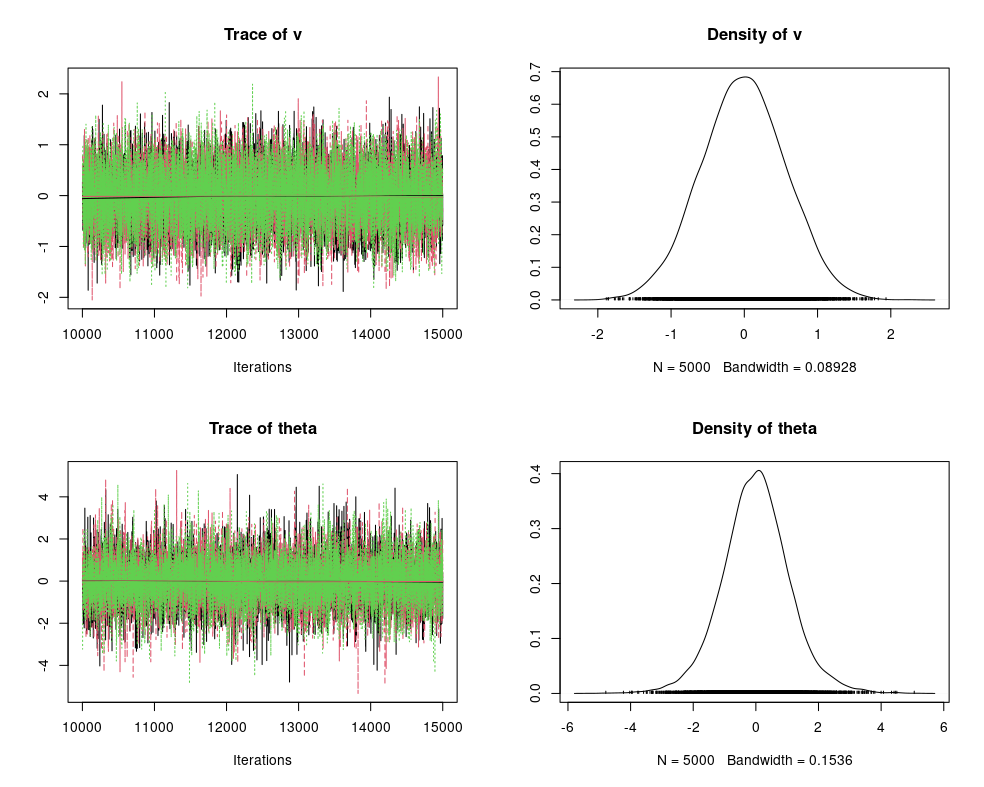
\includegraphics[width=1\linewidth]{1_jags_CE_simple}
	%
	\caption[The Devil's funnel. Centered Parametrization. JAGS]%
	{The Devil's funnel. Centered Parametrization implemented in JAGS. It shows the traceplot and distribution of the parameters of interest.}
	\label{fig:devil_CE_simple_jags}
\end{figure}
%
\begin{figure}[H]
	\centering
	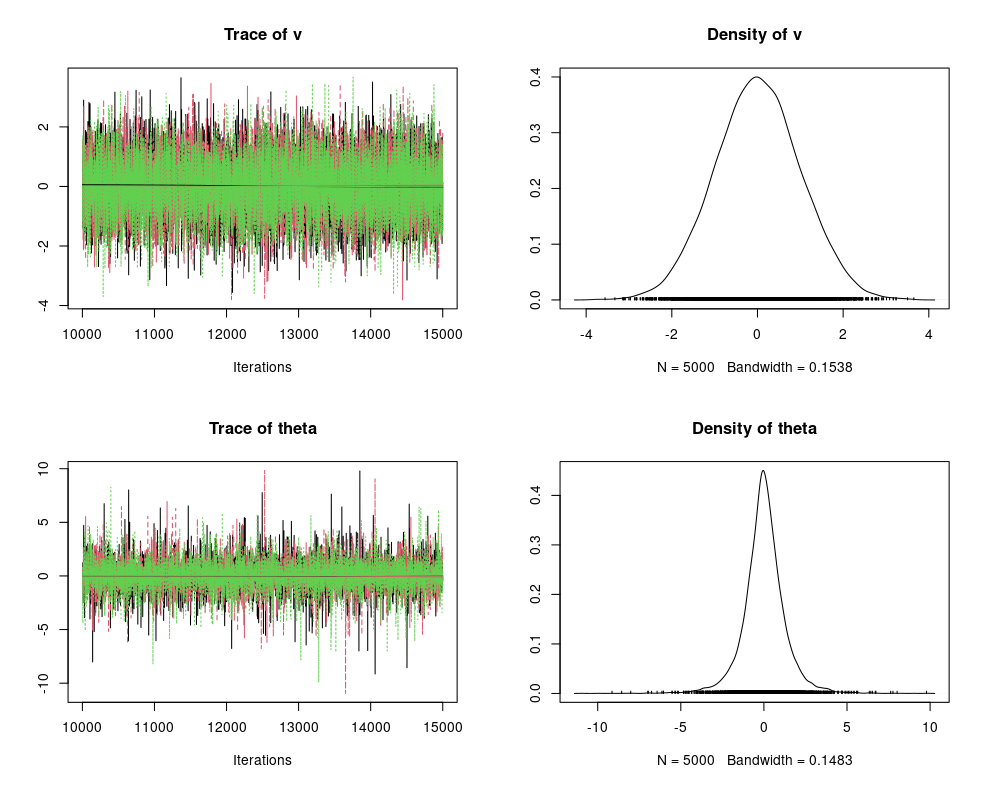
\includegraphics[width=1\linewidth]{2_jags_CE_priors}
	%
	\caption[The Devil's funnel. Centered Parametrization with mildly informative priors. JAGS]%
	{The Devil's funnel. Centered Parametrization with mildly informative priors implemented in JAGS. It shows the traceplot and distribution of the parameters of interest.}
	\label{fig:devil_CE_prior_jags}
\end{figure}
%
\begin{figure}[H]
	\centering
	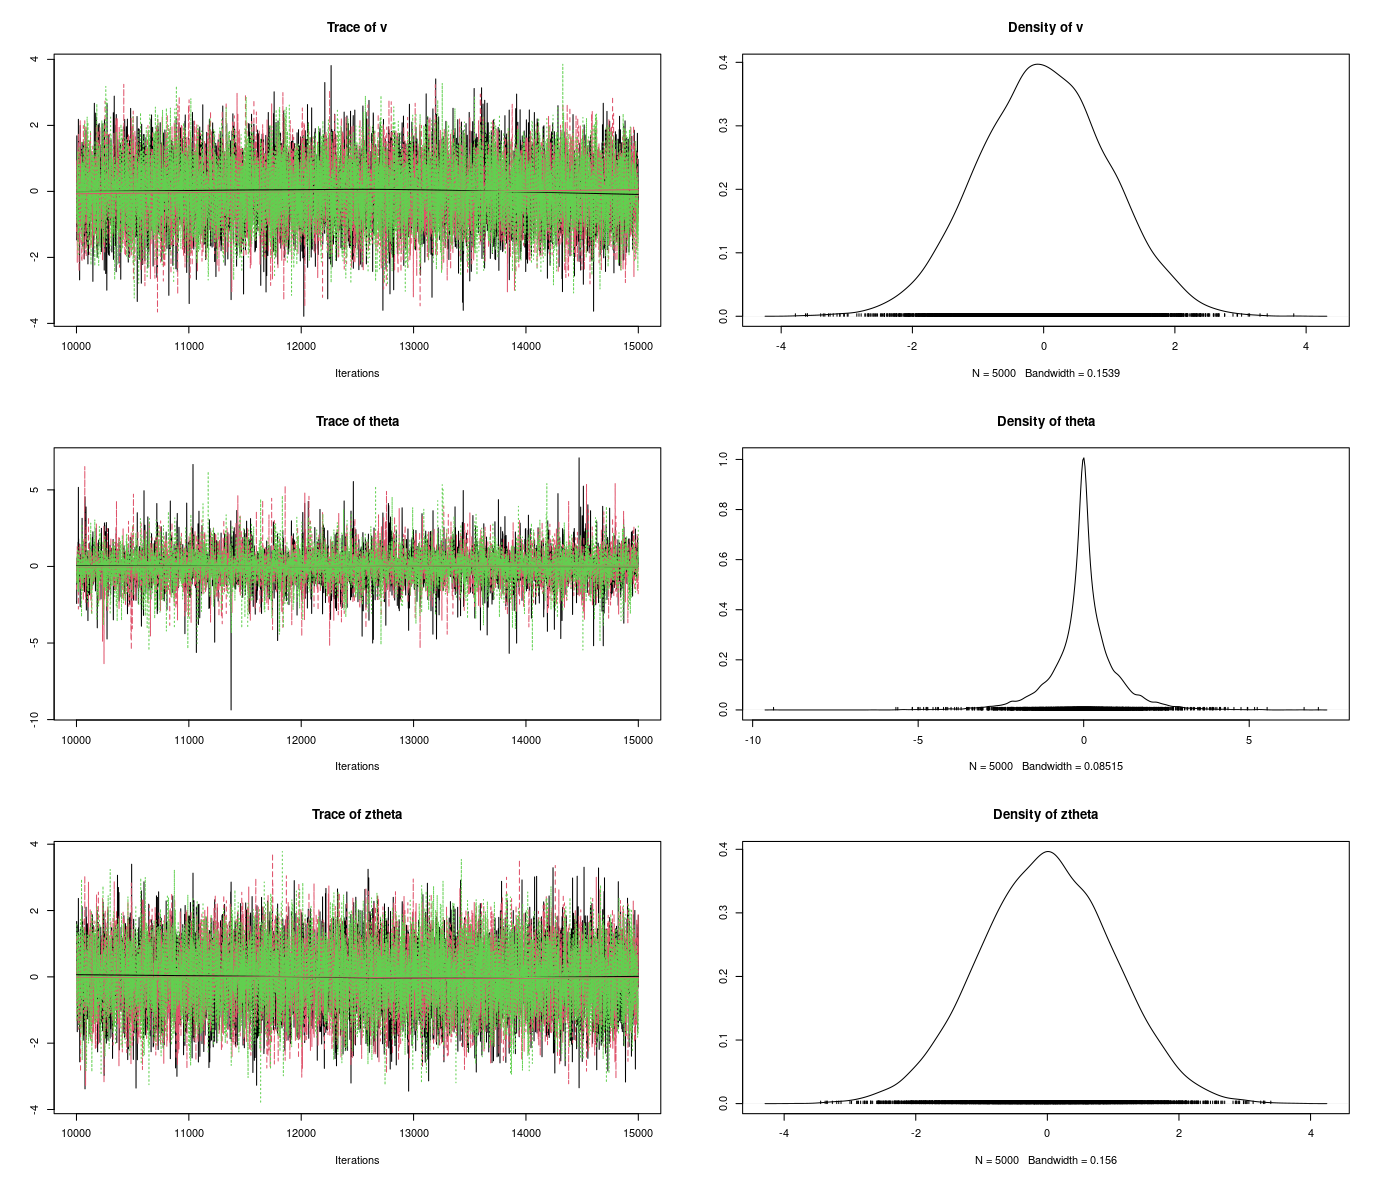
\includegraphics[width=1\linewidth]{3_jags_NC}
	%
	\caption[The Devil's funnel. Non-Centered Parametrization. JAGS]%
	{The Devil's funnel. Non-Centered Parametrization implemented in JAGS. It shows the traceplot and distribution of the parameters of interest.}
	\label{fig:devil_CE_NC_jags}
\end{figure}

%%%%%%%%%%%%%%%%%%%%%%%%%%%%%%%%%%%%%%%%%%%%%%%%%%%%%%%%%%%%%%%%%%%%%%%


%%%%%%%%%%%%%%%%%%%%%%%%%%%%%%%%%%%%%%%%%%%%%%%%%%%%%%%%%%%%%%%%%%%%%%%
%%%%%%%%%%%%%%%%%%%%%%%%%%%%%%%%%%%%%%%%%%%%%%%%%%%%%%%%%%%%%%%%%%%%%%%


\section{Chapter 4: Simulation study} \label{appB2:chapter4}

\subsection{Prior elicitation}
%
\begin{figure}[H]
	\centering
	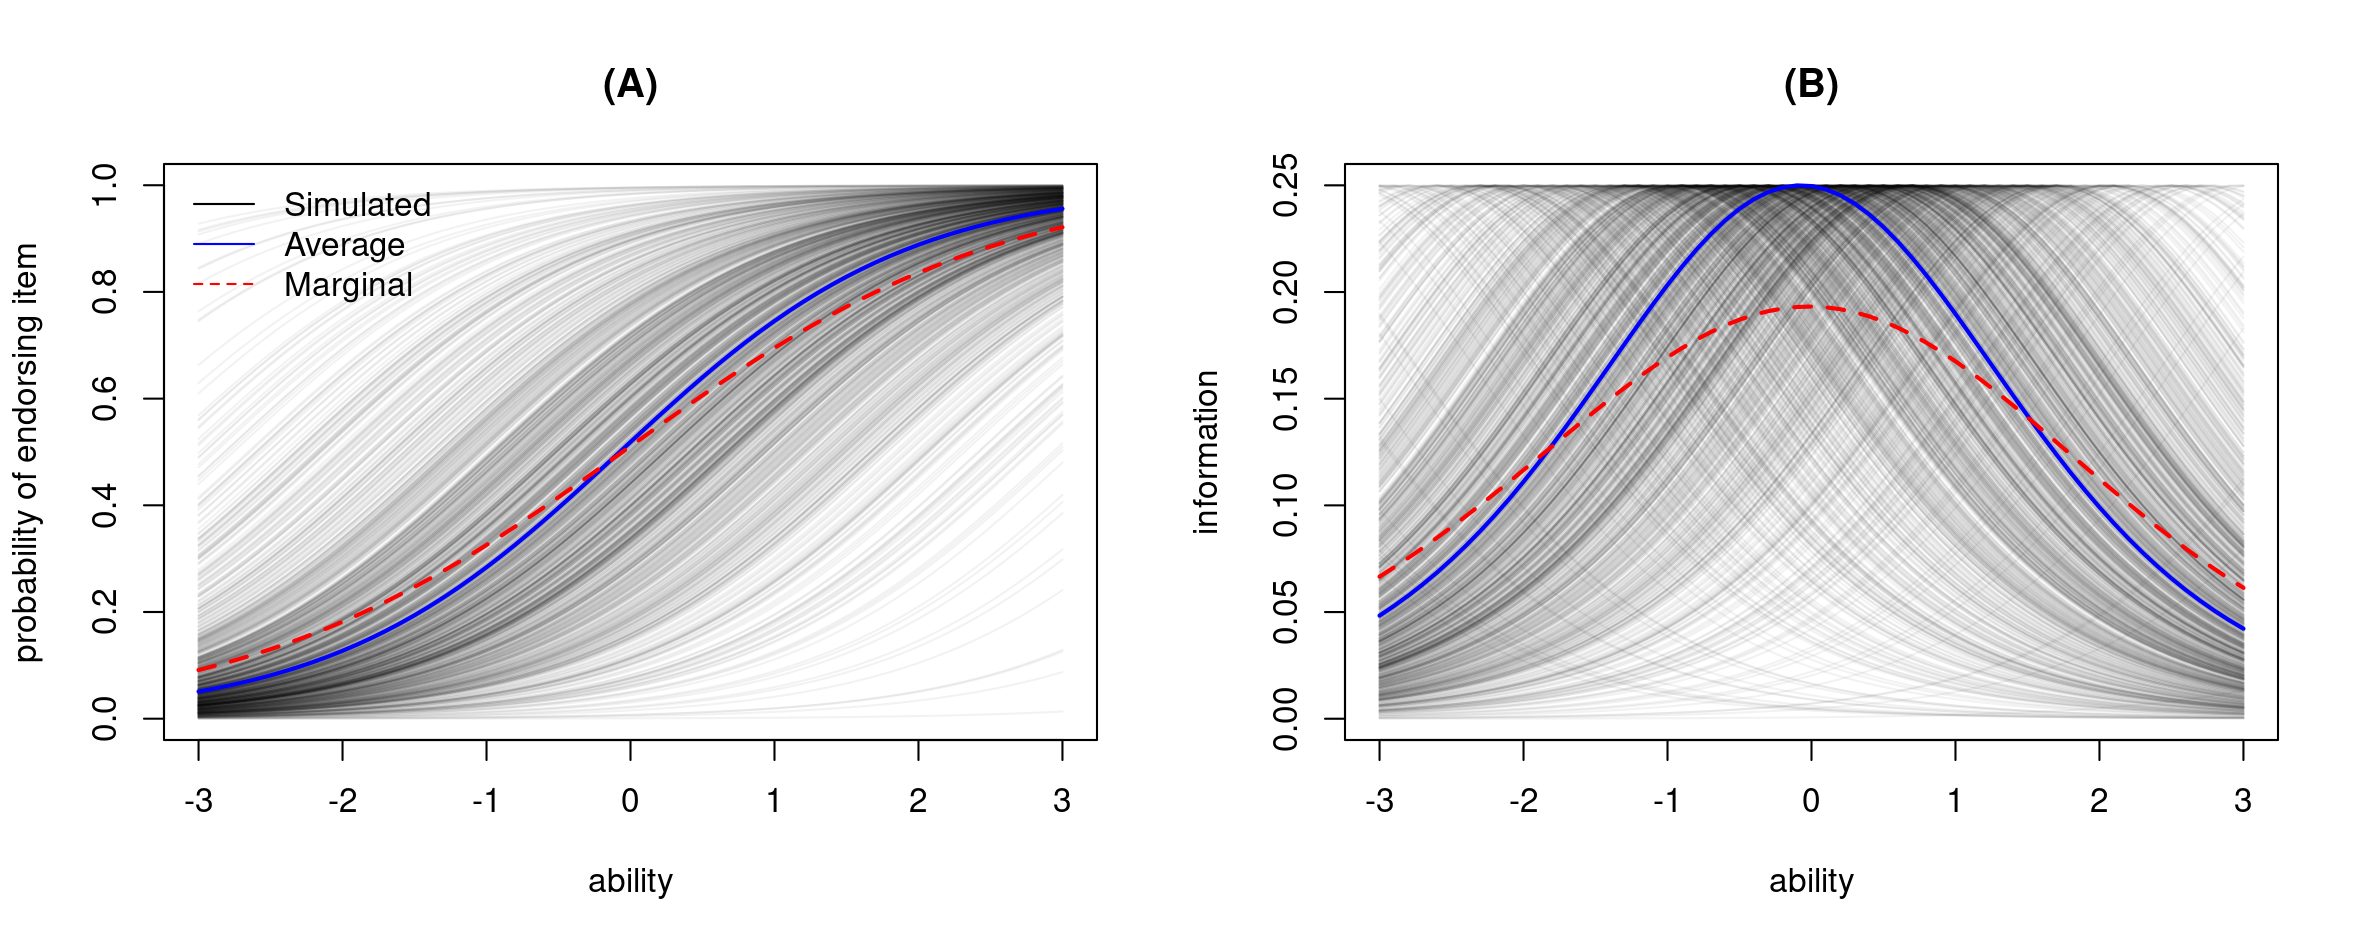
\includegraphics[width=1\linewidth]{SOLV_ICC_prior}
	%
	\caption[Second-Order latent variable model (SOLV). Item Characteristic Curve (ICC) and Item Information Function (IIF).]%
	{Second-Order latent variable model (SOLV). (A) Item Characteristics Curve, ICC. (B) Item Information Function, IIF.}
	\label{fig:SOLV_ICC_prior}
\end{figure}
%
\begin{figure}[H]
	\centering
	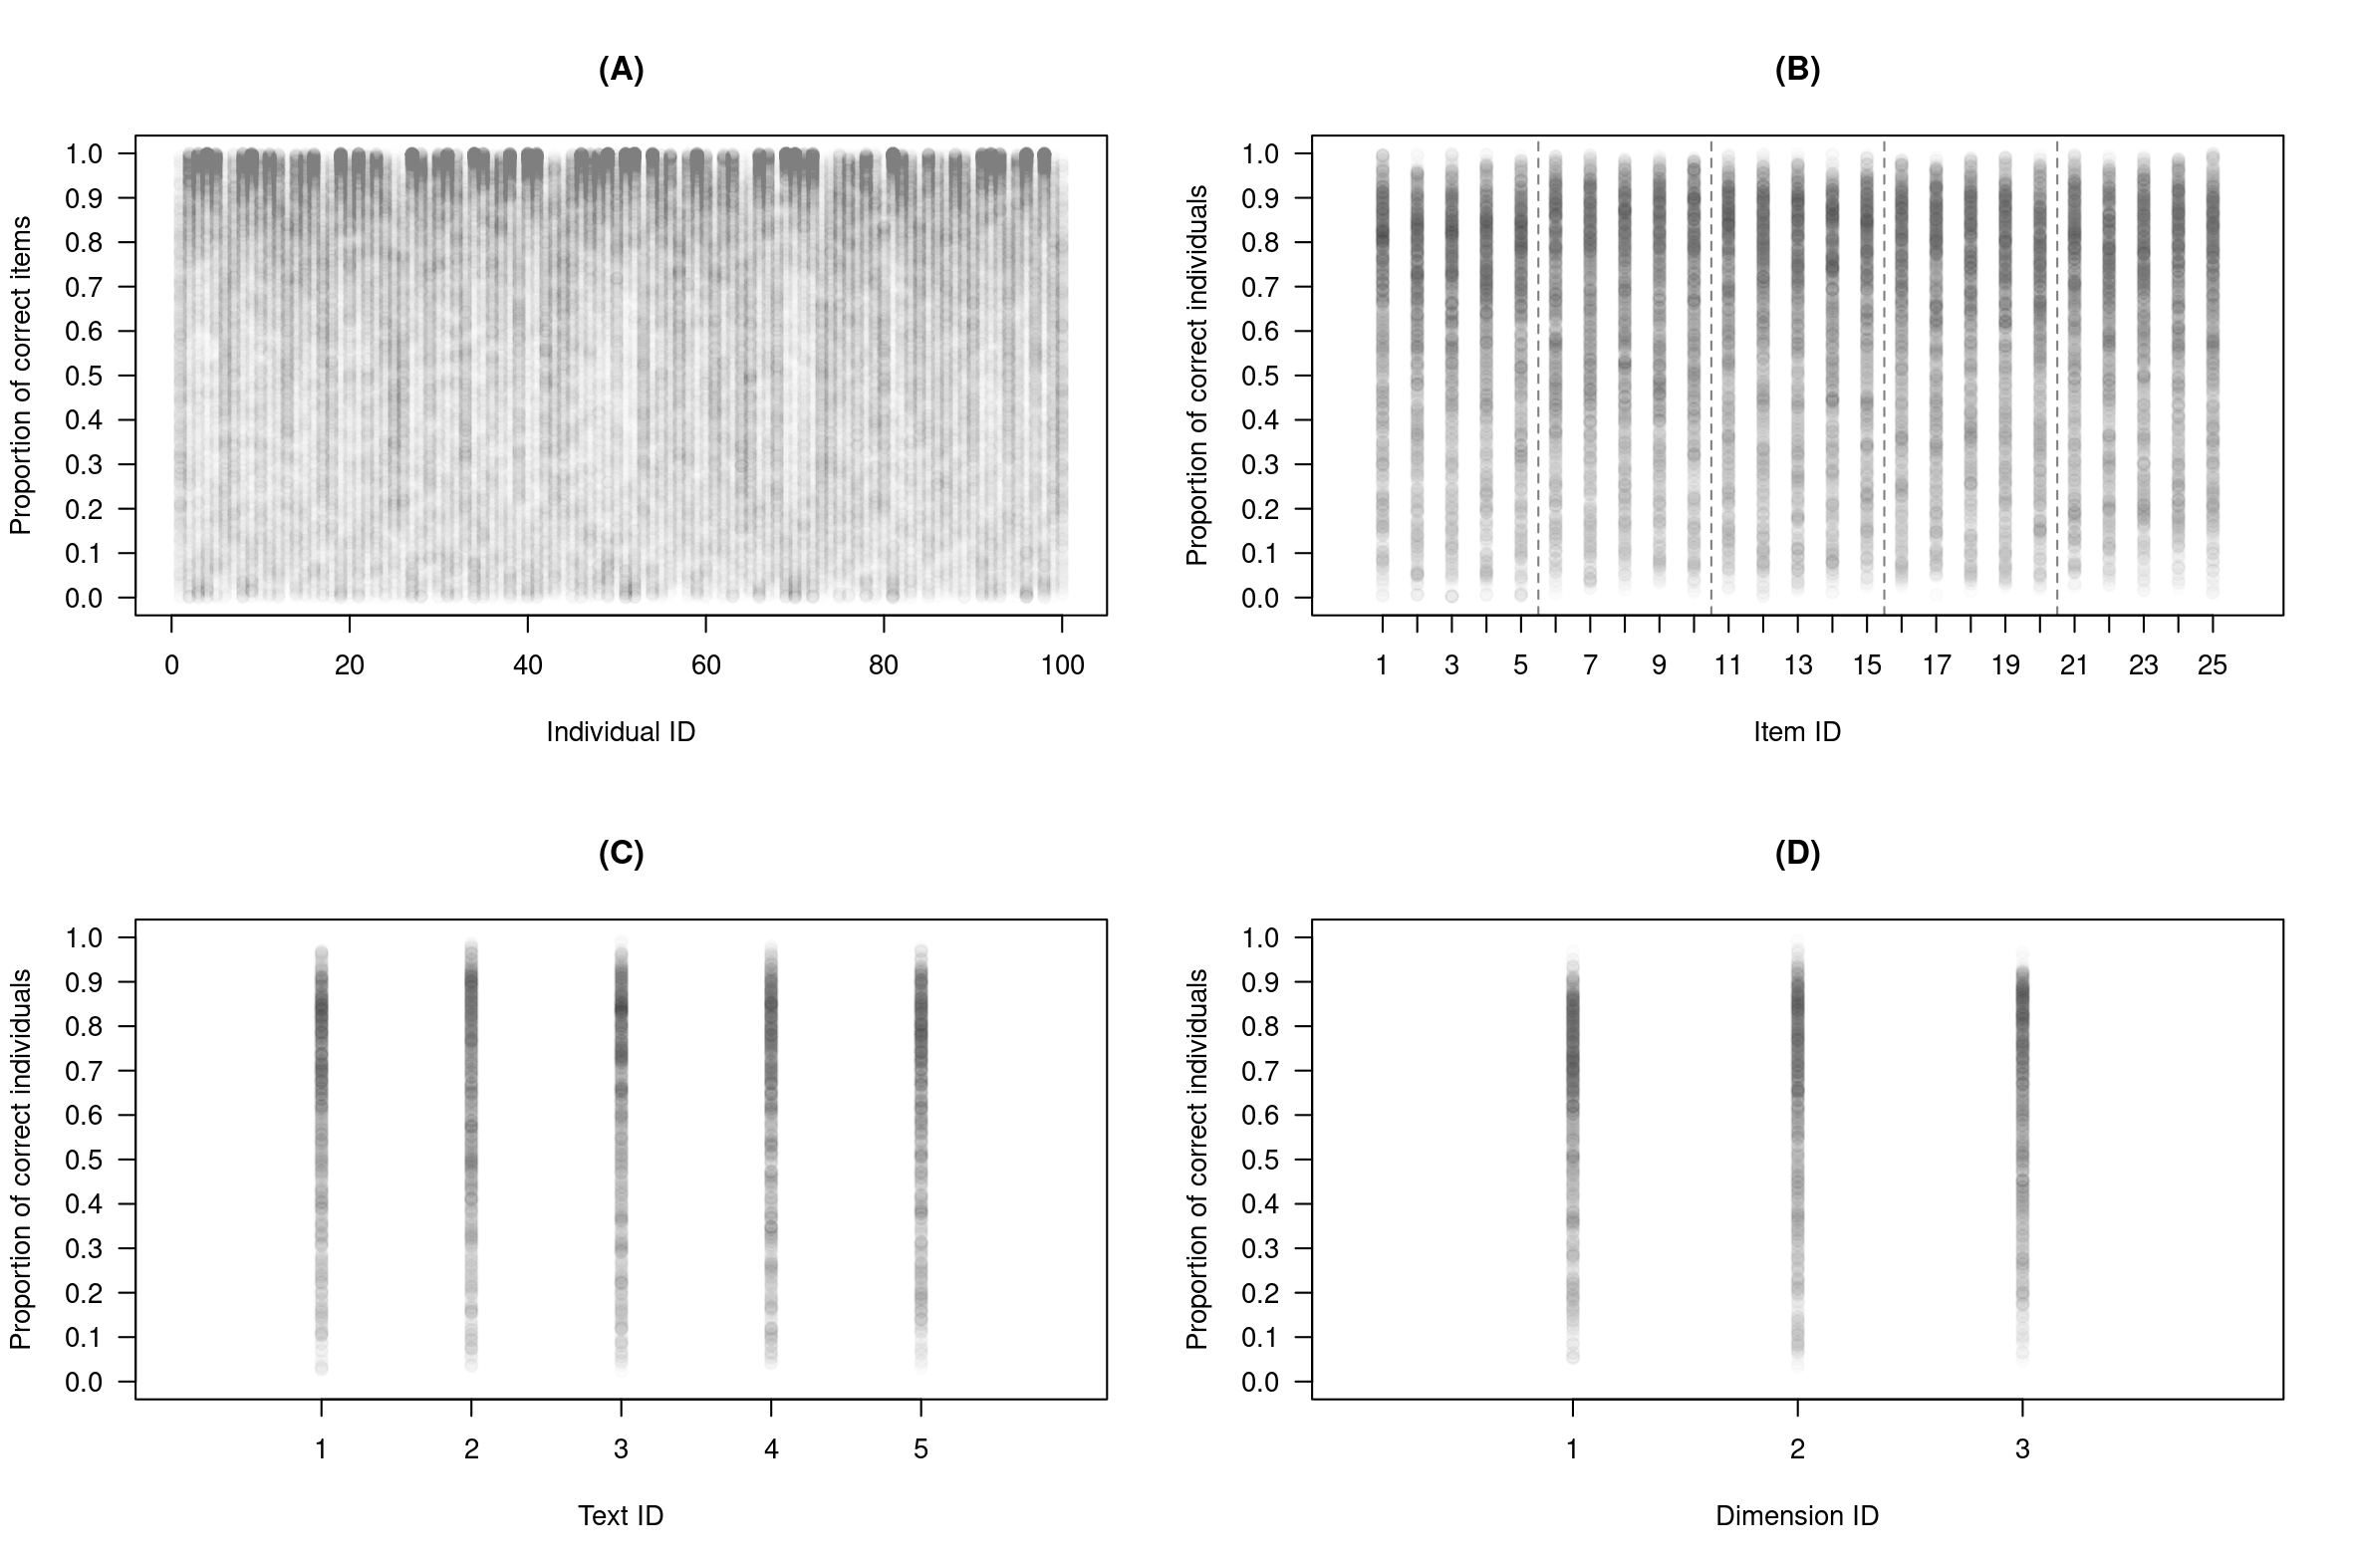
\includegraphics[width=1\linewidth]{SOLV_HitRate1}
	%
	\caption[Second-Order latent variable model (SOLV). Hit rate per dimensions of interest.]%
	{Second-Order latent variable model (SOLV). Aggregated endorsement rate per: (A) individuals, (B) items, (C) text or passage, and (D) measured dimension.}
	\label{fig:SOLV_hitrate1}
\end{figure}
%
\begin{figure}[H]
	\centering
	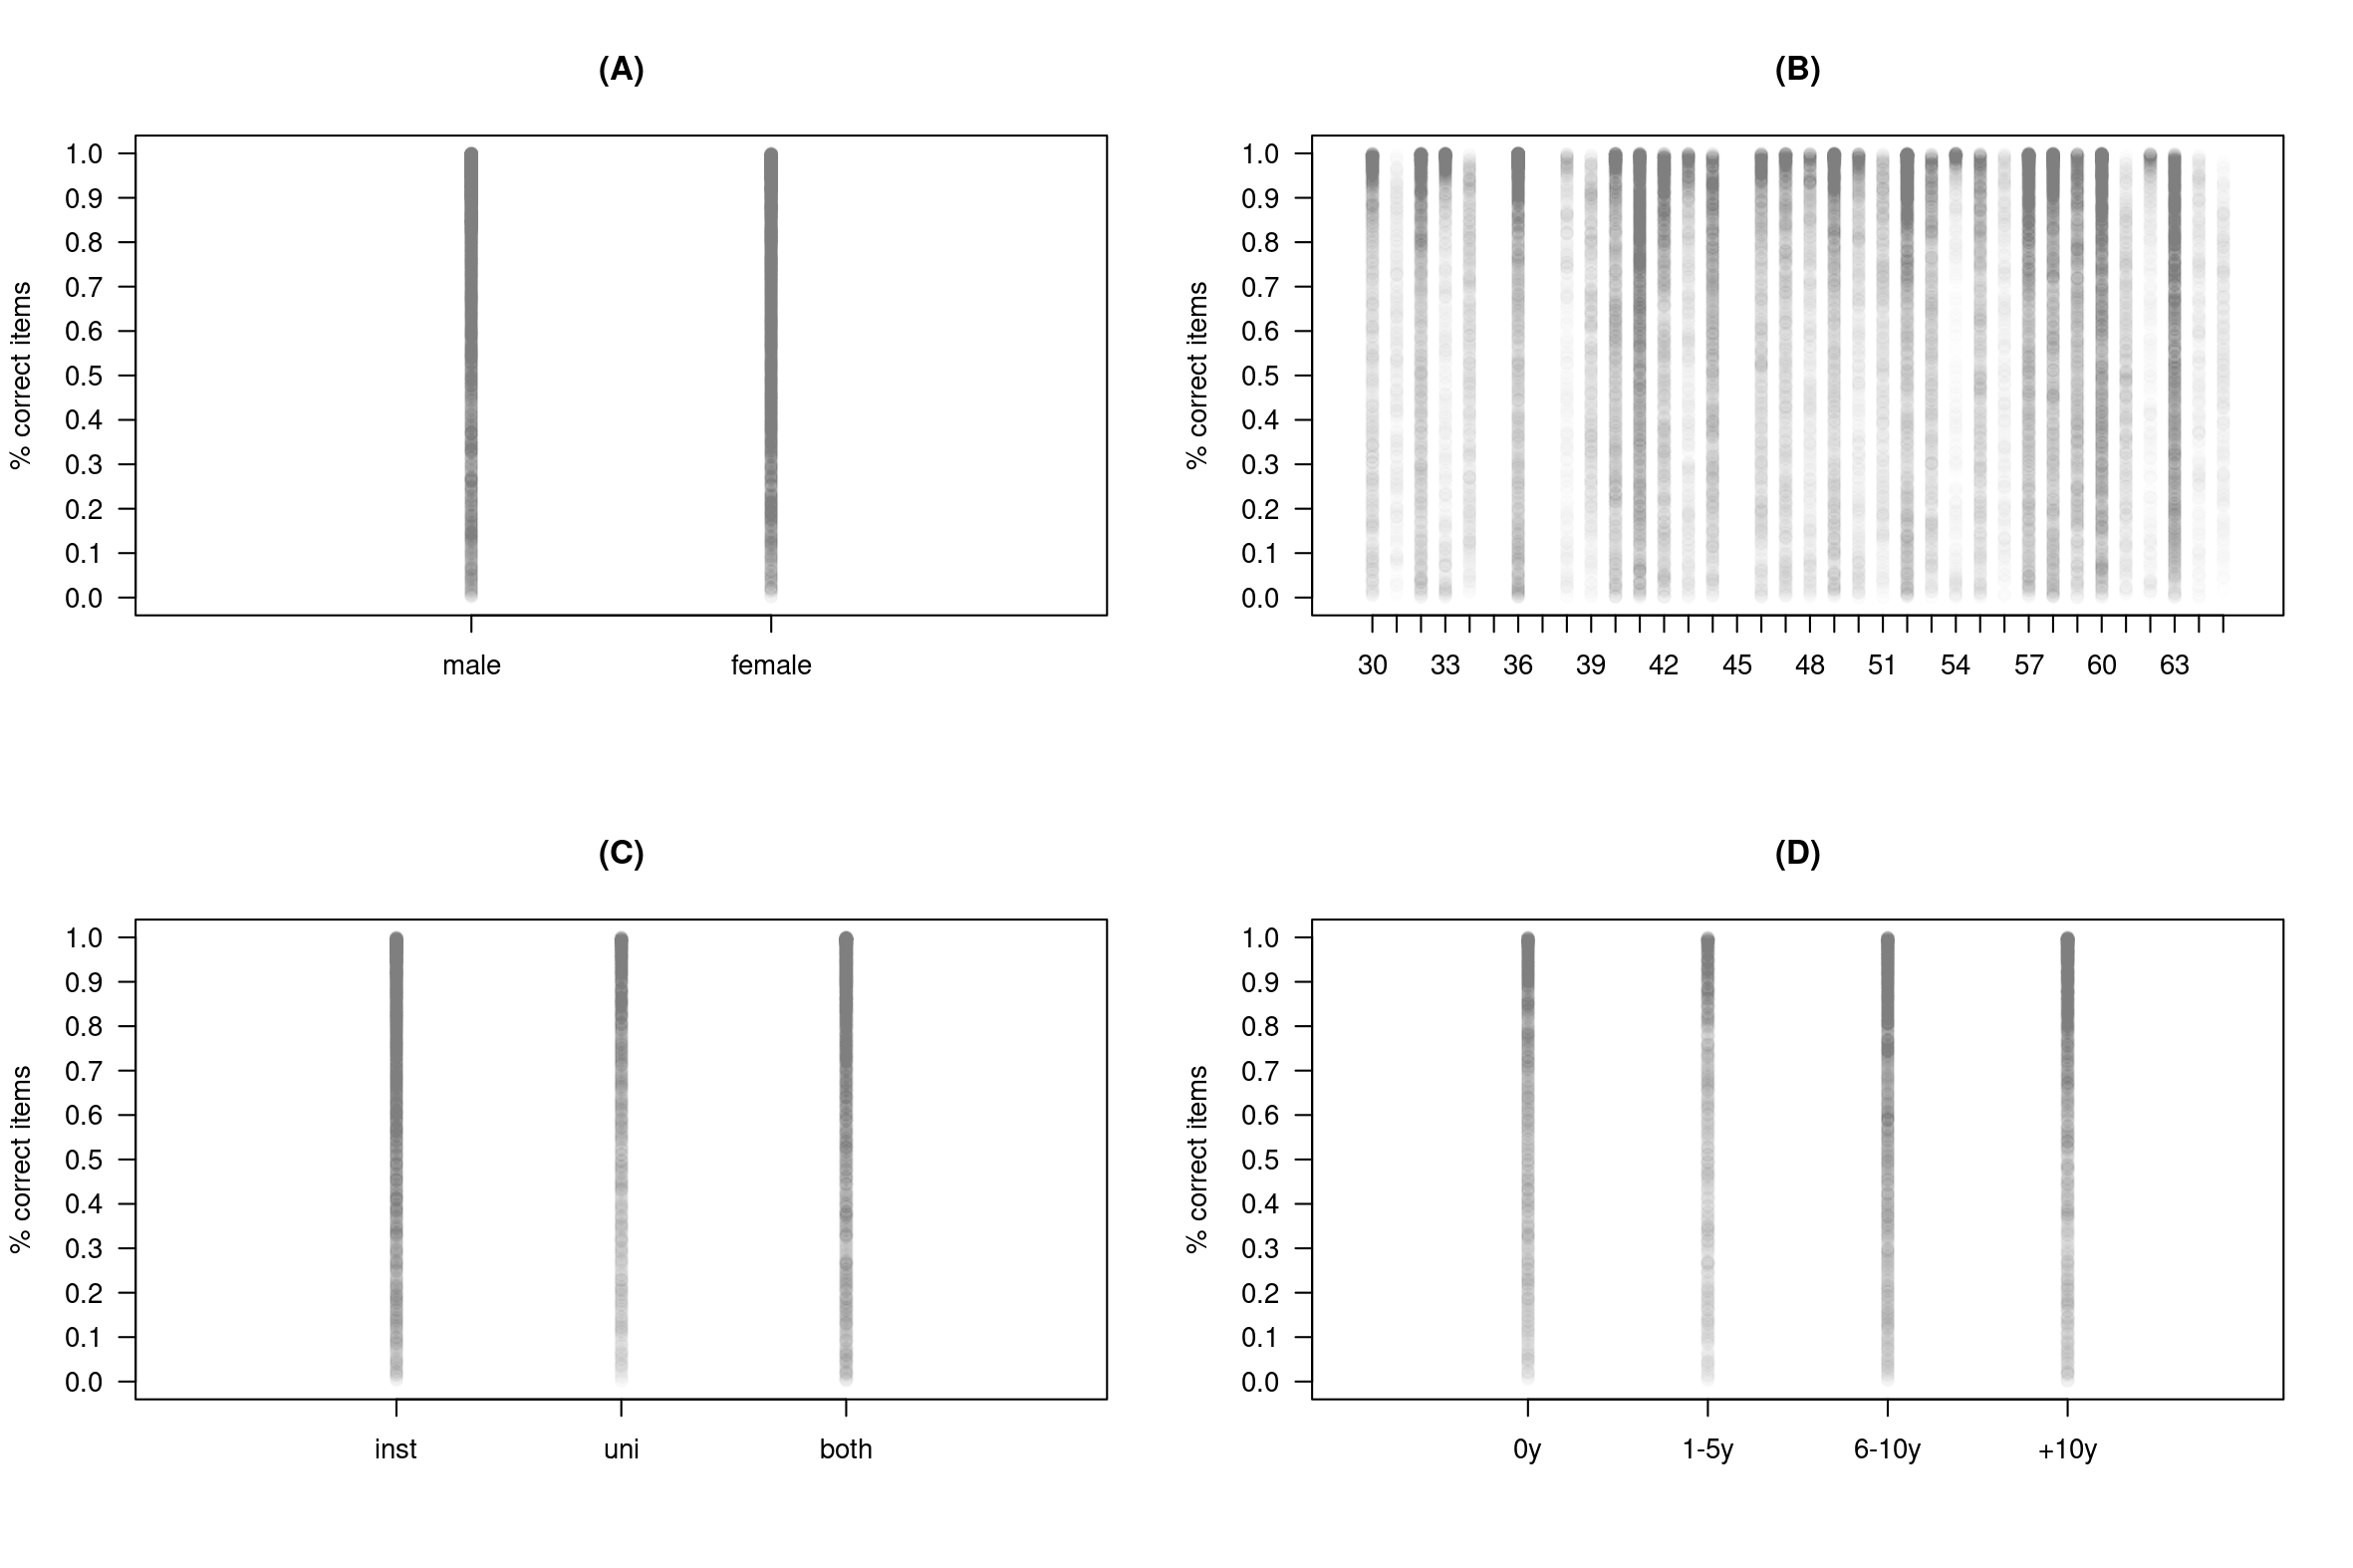
\includegraphics[width=1\linewidth]{SOLV_HitRate2}
	%
	\caption[Second-Order latent variable model (SOLV). Hit rate per simulated covariate.]%
	{Second-Order latent variable model (SOLV). Aggregated endorsement rate per simulated covariate: (A) gender, (B) age, (C) education, and (D) experience.}
	\label{fig:SOLV_hitrate2}
\end{figure}


\subsection{Chain performance}

Trace, trank and ACF plots for all models, parametrizations, and replicas can be found in the images section of the accompanying github page:

\noindent \url{https://github.com/jriveraespejo/thesis/tree/master/images/chains} \\

\noindent The CP and NCP comparison plots of effective sample sizes (\texttt{n\_eff}) and \texttt{Rhat}, for both models (across replicas), can be found in the corresponding image section of the accompanying github page:

\noindent \url{https://github.com/jriveraespejo/thesis/tree/master/images/chains_stat}
%
\begin{figure}[H]
	\centering
	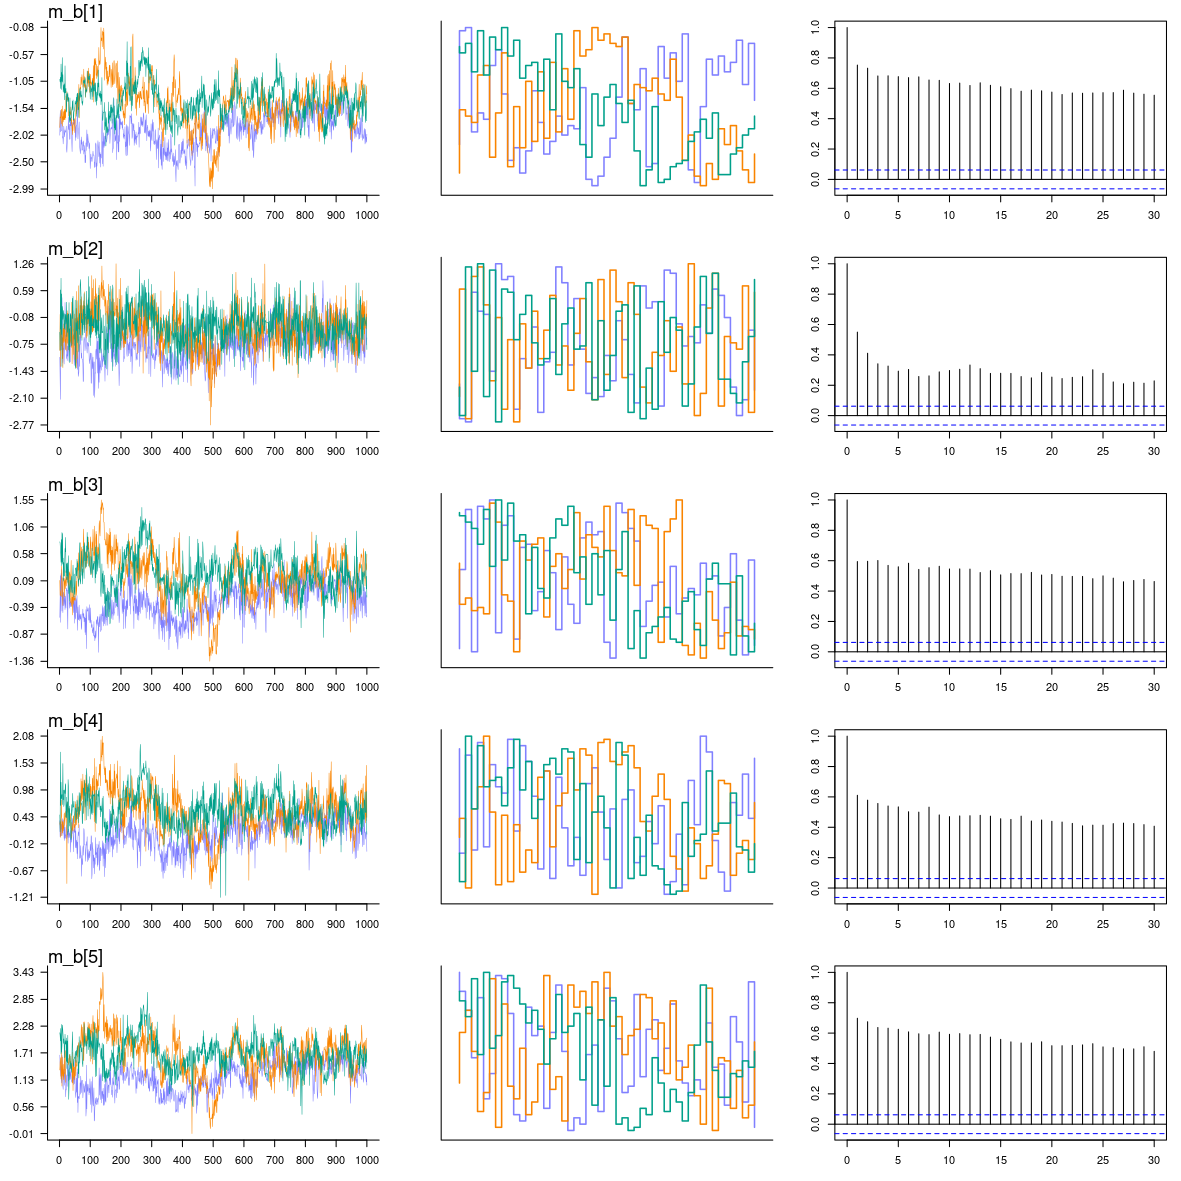
\includegraphics[width=1\linewidth]{FOLV_CE_J100_Ndata2_mb}
	%
	\caption[First-Order latent variable model (FOLV). Centered parametrization. Mean difficulty per text. Trace, trank and auto-correlation plots.]%
	{First-Order latent variable model (FOLV). Centered parametrization. Mean difficulty per text: (Left) trace plot, (Middle) trank plot, (Right) auto-correlation plot.}
	\label{fig:FOLV_CE_chains1}
\end{figure}
%
\begin{figure}[H]
	\centering
	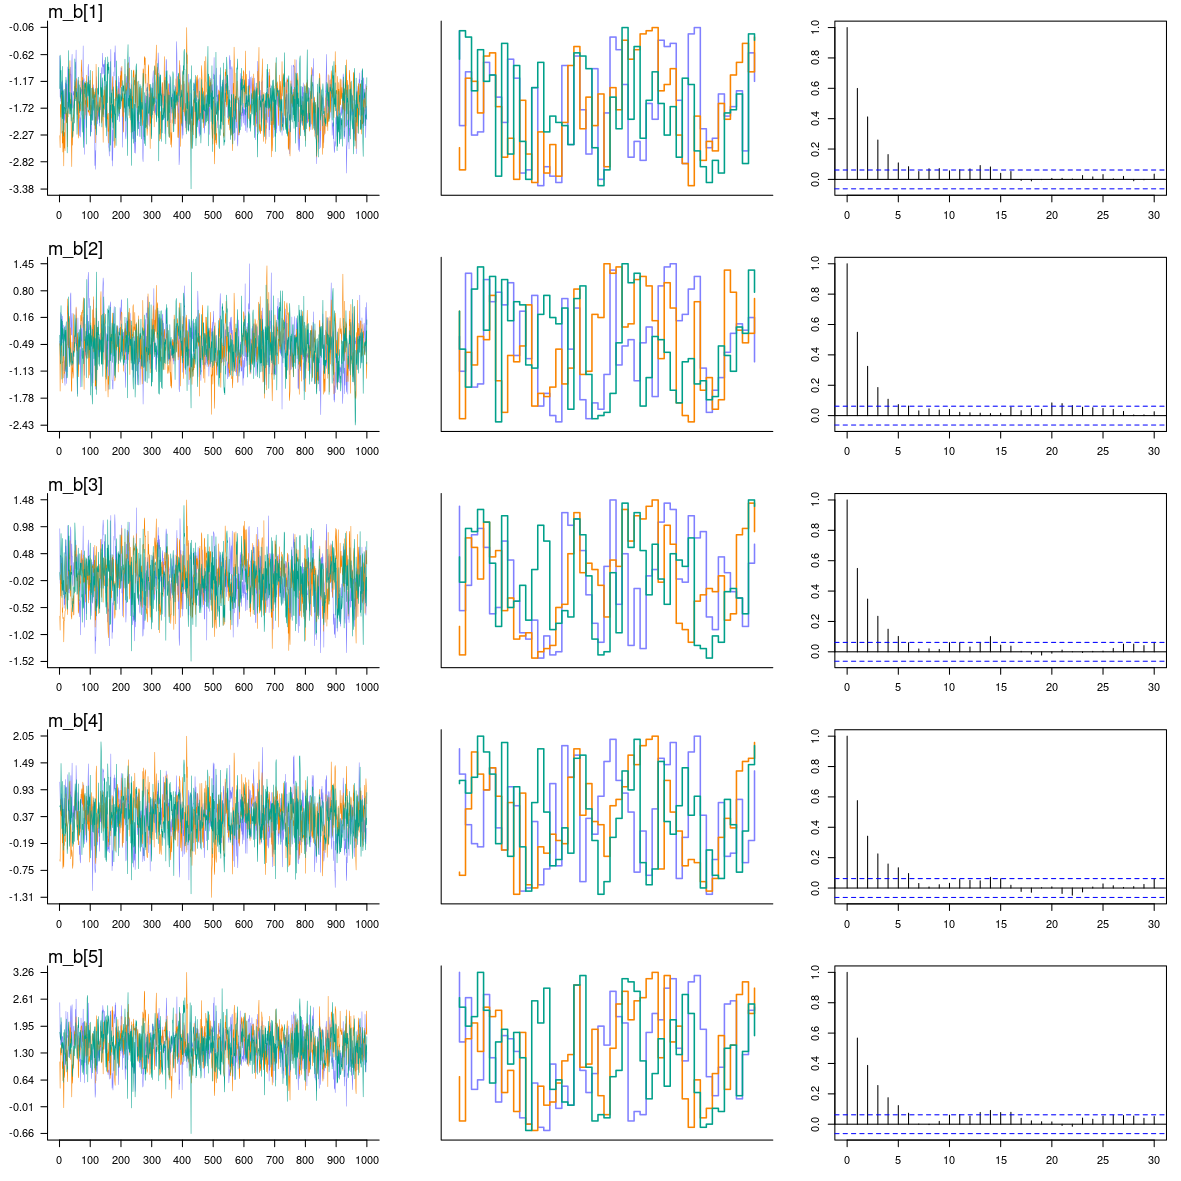
\includegraphics[width=1\linewidth]{FOLV_NC_J100_Ndata2_mb}
	%
	\caption[First-Order latent variable model (FOLV). Non-centered parametrization. Mean difficulty per text. Trace, trank and auto-correlation plots.]%
	{First-Order latent variable model (FOLV). Non-centered parametrization. Mean difficulty per text: (Left) trace plot, (Middle) trank plot, (Right) auto-correlation plot.}
	\label{fig:FOLV_NC_chains1}
\end{figure}
%
\begin{figure}[H]
	\centering
	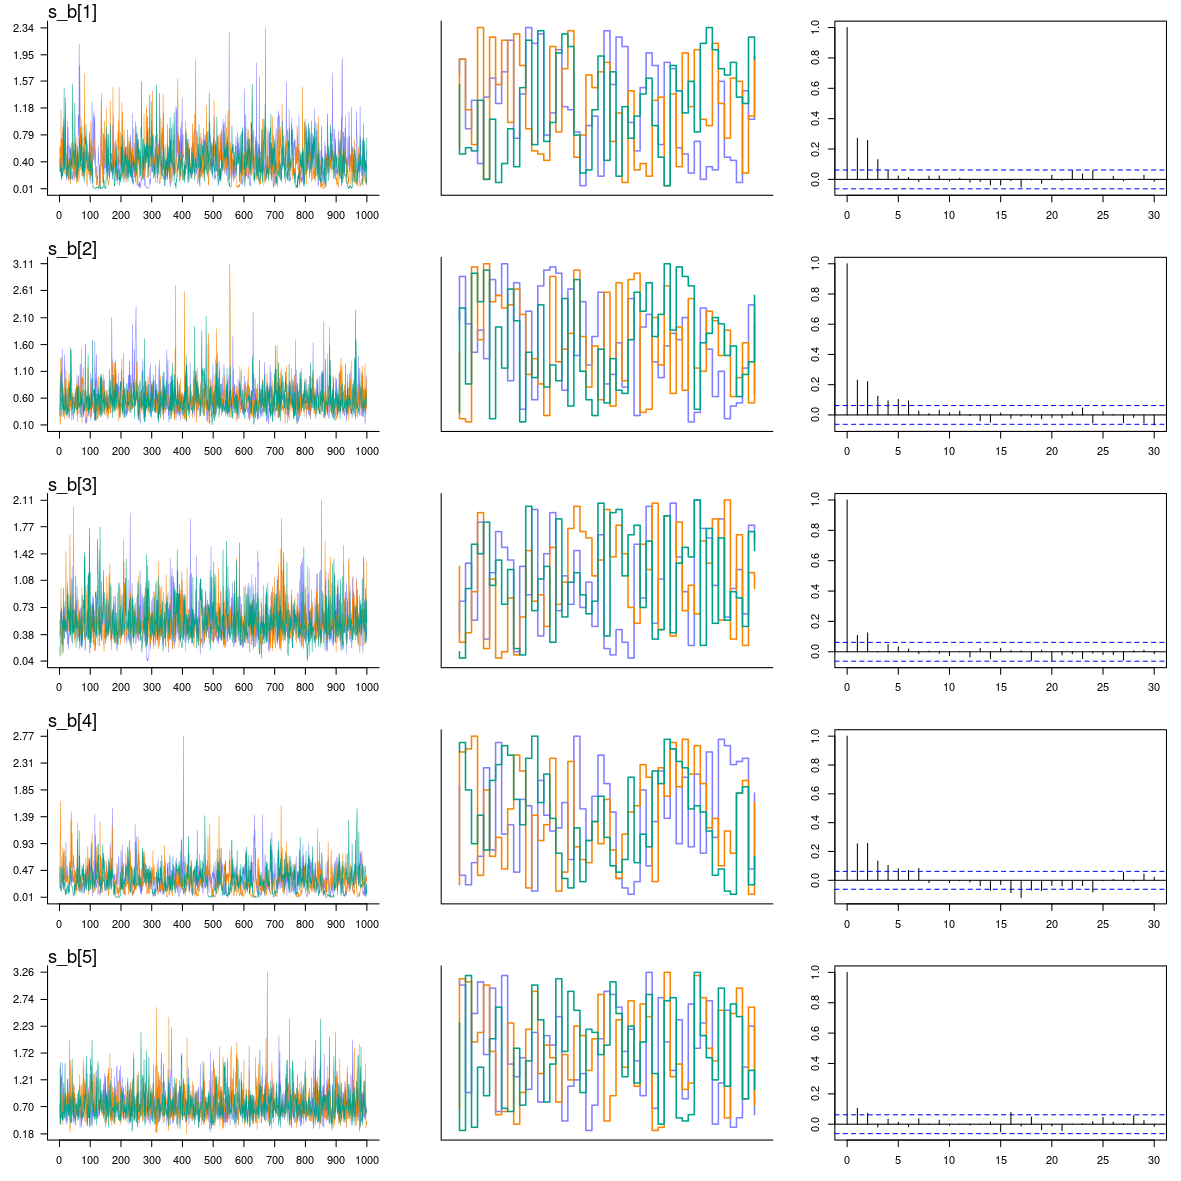
\includegraphics[width=1\linewidth]{FOLV_CE_J100_Ndata3_sb}
	%
	\caption[First-Order latent variable model (FOLV). Centered parametrization. Difficulty deviation per text. Trace, trank and auto-correlation plots.]%
	{First-Order latent variable model (FOLV). Centered parametrization. Difficulty deviation per text: (Left) trace plot, (Middle) trank plot, (Right) auto-correlation plot.}
	\label{fig:FOLV_CE_chains2}
\end{figure}
%
\begin{figure}[H]
	\centering
	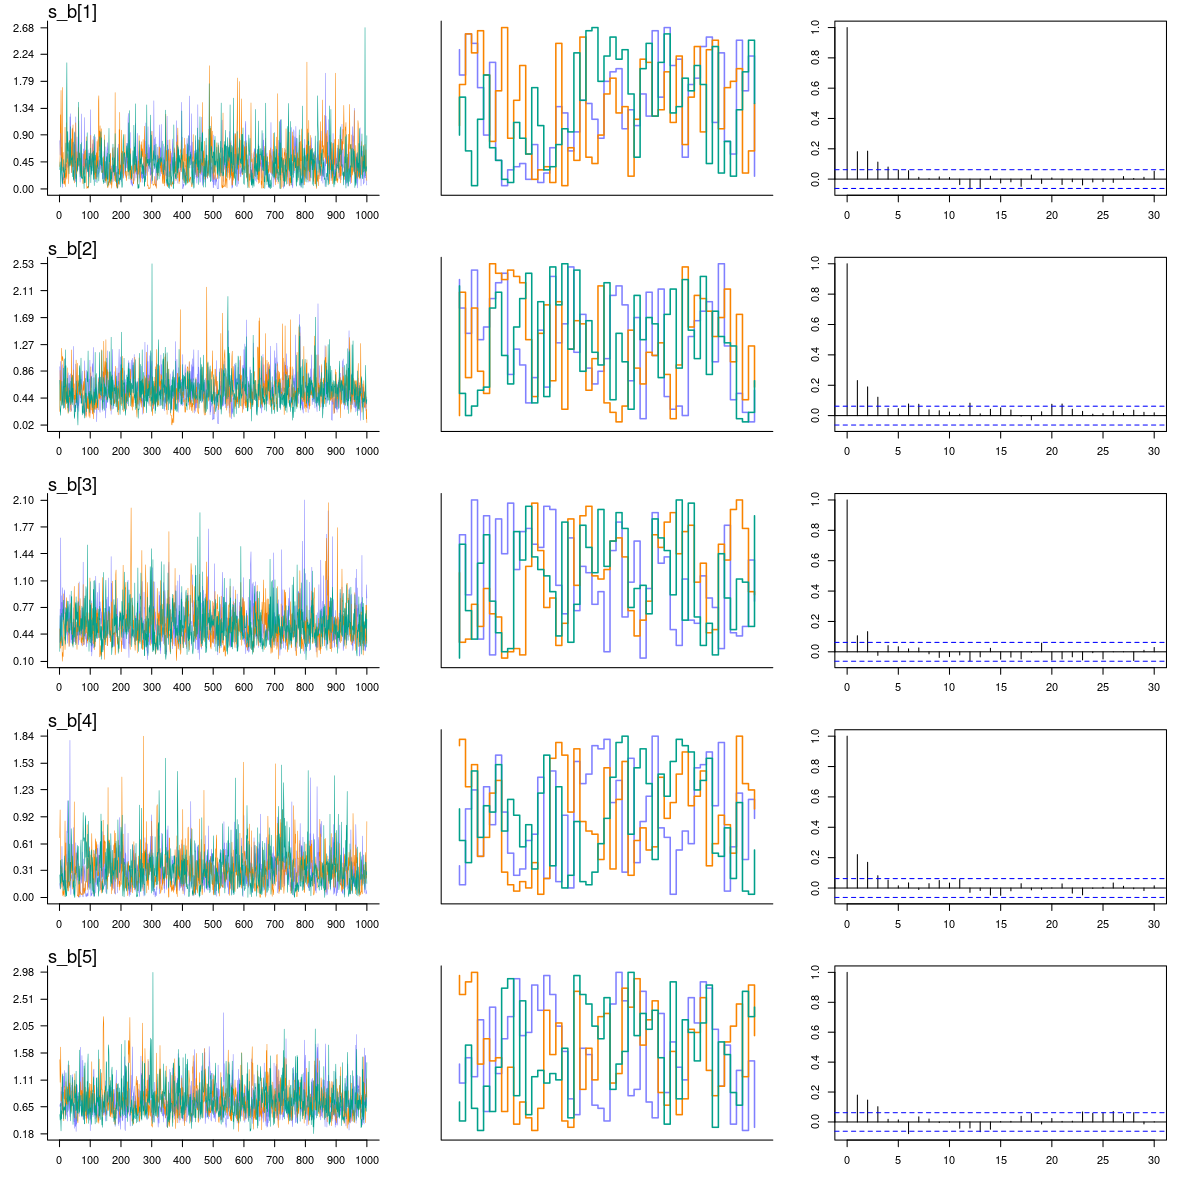
\includegraphics[width=1\linewidth]{FOLV_NC_J100_Ndata3_sb}
	%
	\caption[First-Order latent variable model (FOLV). Non-centered parametrization. Difficulty deviation per text. Trace, trank and auto-correlation plots.]%
	{First-Order latent variable model (FOLV). Non-centered parametrization. Difficulty deviation per text: (Left) trace plot, (Middle) trank plot, (Right) auto-correlation plot.}
	\label{fig:FOLV_NC_chains2}
\end{figure}
%
\begin{figure}[H]
	\centering
	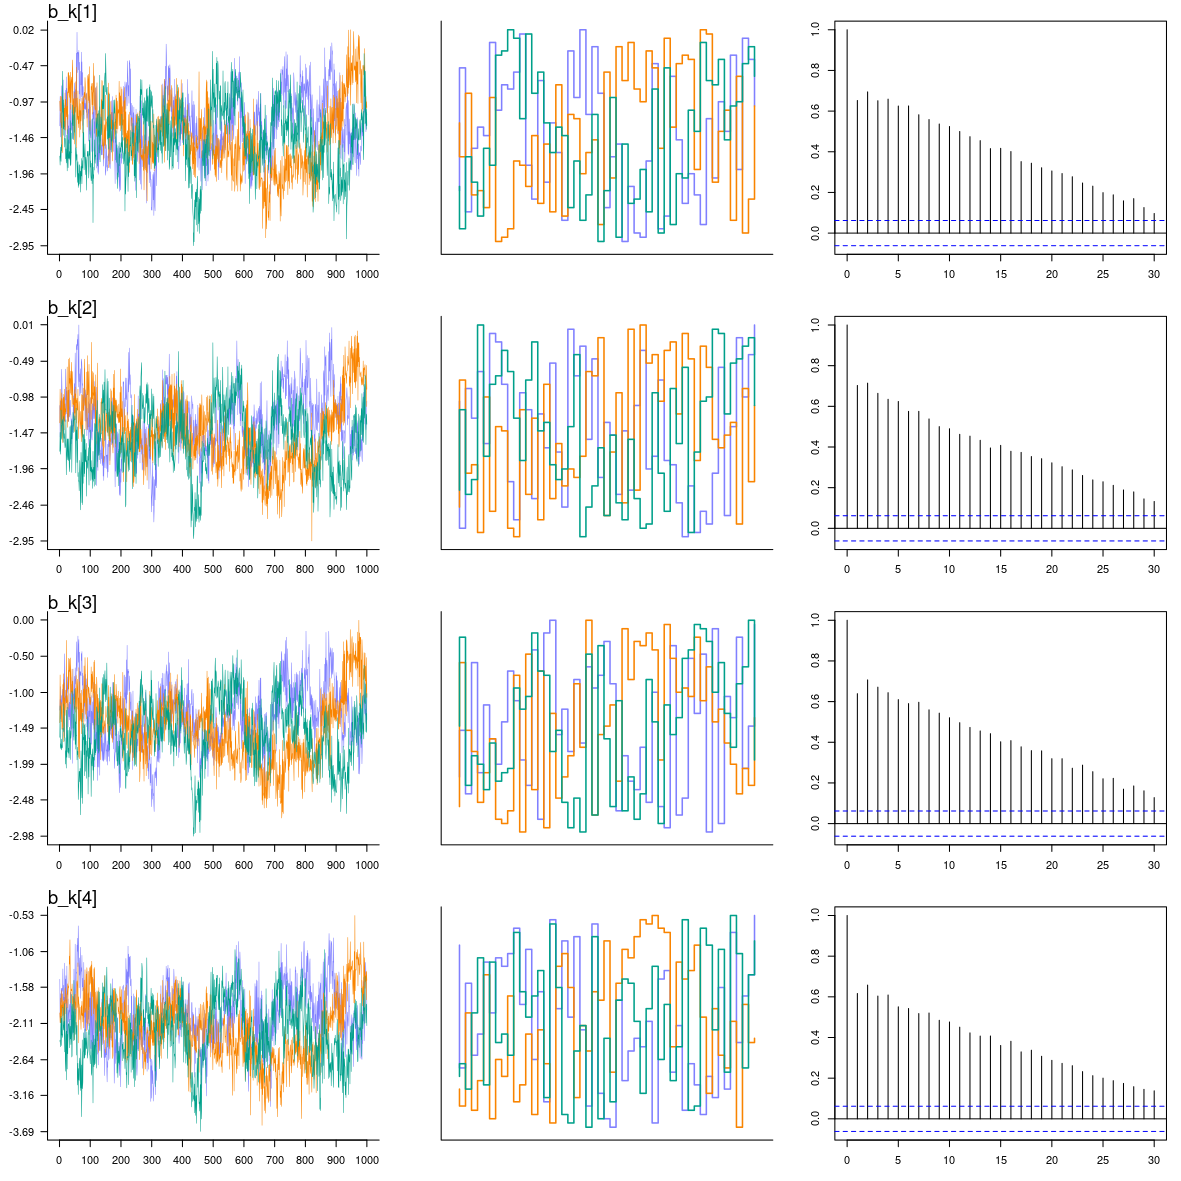
\includegraphics[width=1\linewidth]{FOLV_CE_J100_Ndata1_bk1}
	%
	\caption[First-Order latent variable model (FOLV). Centered parametrization. Difficulty per item. Trace, trank and auto-correlation plots.]%
	{First-Order latent variable model (FOLV). Centered parametrization. Difficulty per item: (Left) trace plot, (Middle) trank plot, (Right) auto-correlation plot.}
	\label{fig:FOLV_CE_chains3}
\end{figure}
%
\begin{figure}[H]
	\centering
	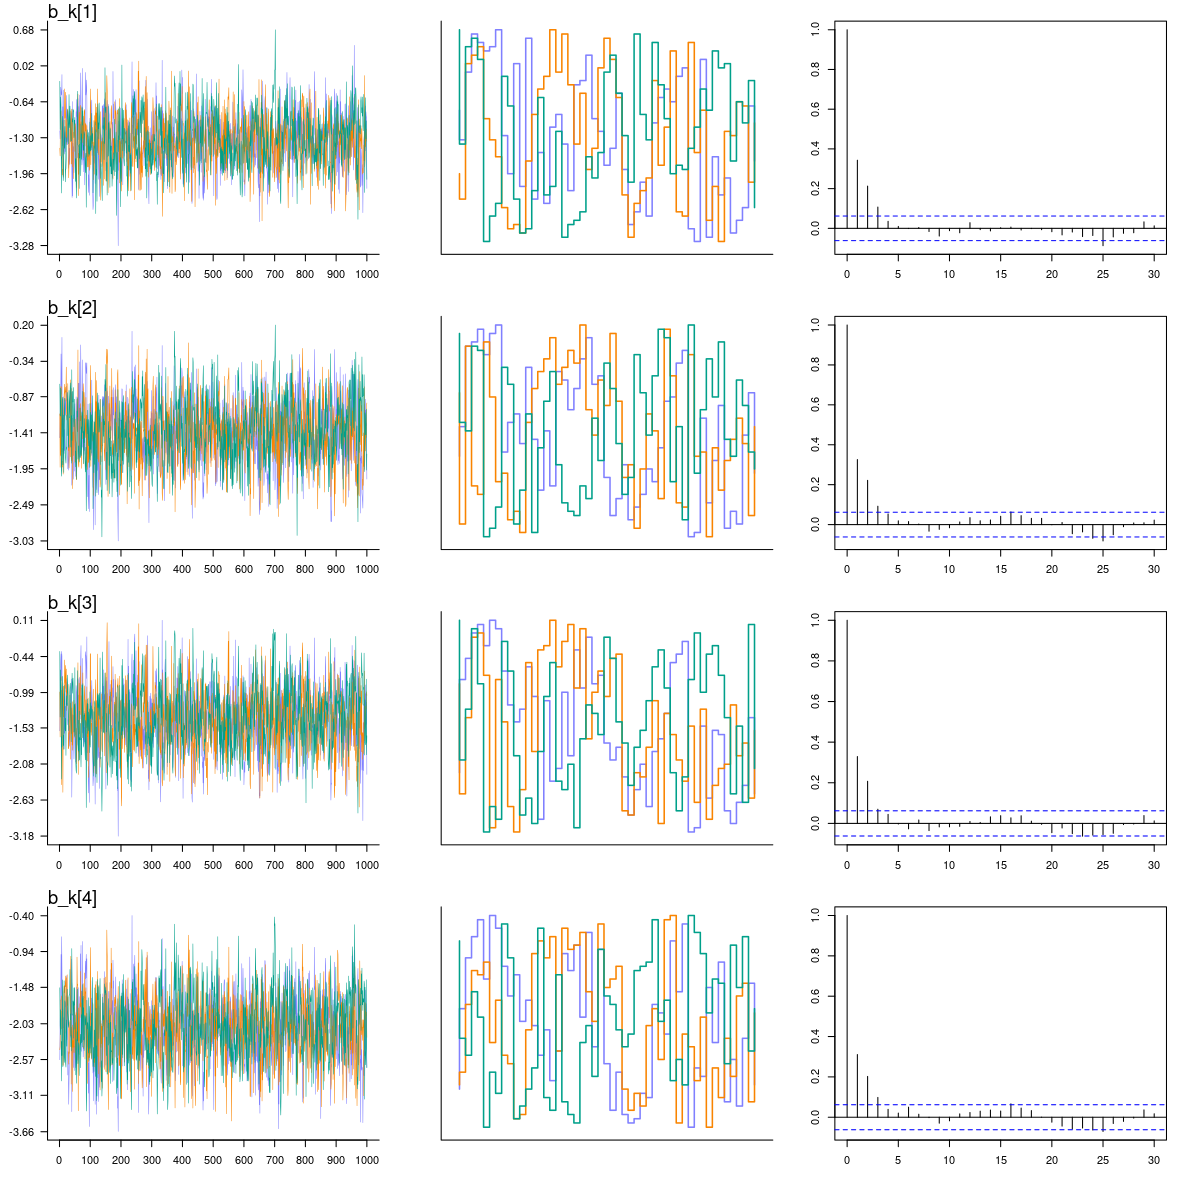
\includegraphics[width=1\linewidth]{FOLV_NC_J100_Ndata1_bk1}
	%
	\caption[First-Order latent variable model (FOLV). Non-centered parametrization. Difficulty per item. Trace, trank and auto-correlation plots.]%
	{First-Order latent variable model (FOLV). Non-centered parametrization. Difficulty per item: (Left) trace plot, (Middle) trank plot, (Right) auto-correlation plot.}
	\label{fig:FOLV_NC_chains3}
\end{figure}
%
\begin{figure}[H]
	\centering
	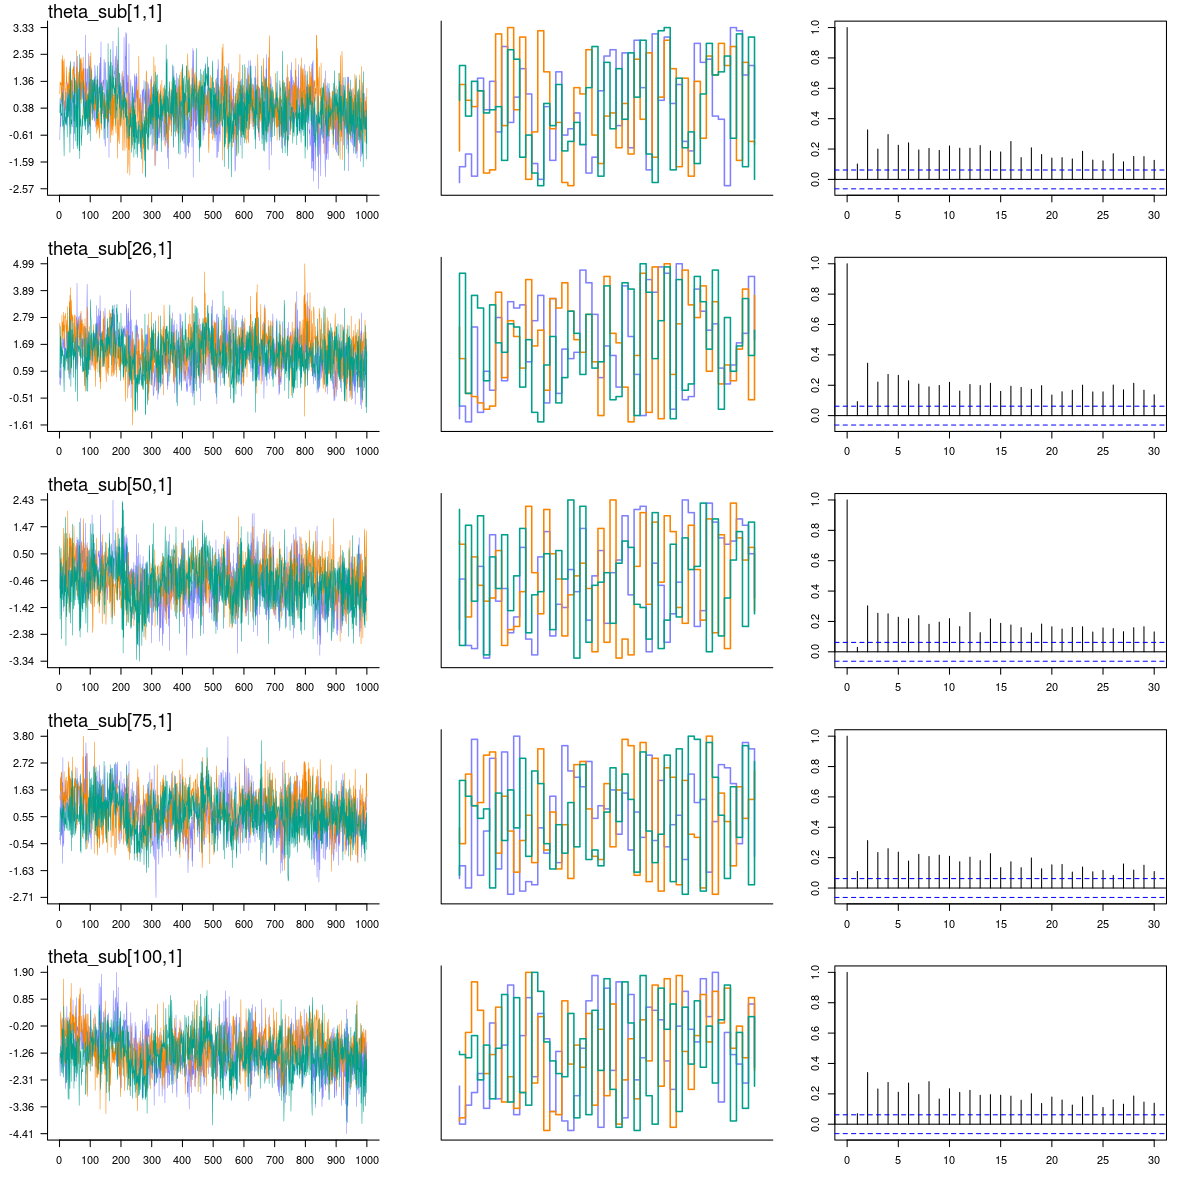
\includegraphics[width=1\linewidth]{FOLV_CE_J100_Ndata6_theta_sub1}
	%
	\caption[First-Order latent variable model (FOLV). Centered parametrization. Individual's first sub-dimension. Trace, trank and auto-correlation plots.]%
	{First-Order latent variable model (FOLV). Centered parametrization. Individual's first sub-dimension: (Left) trace plot, (Middle) trank plot, (Right) auto-correlation plot.}
	\label{fig:FOLV_CE_chains4}
\end{figure}
%
\begin{figure}[H]
	\centering
	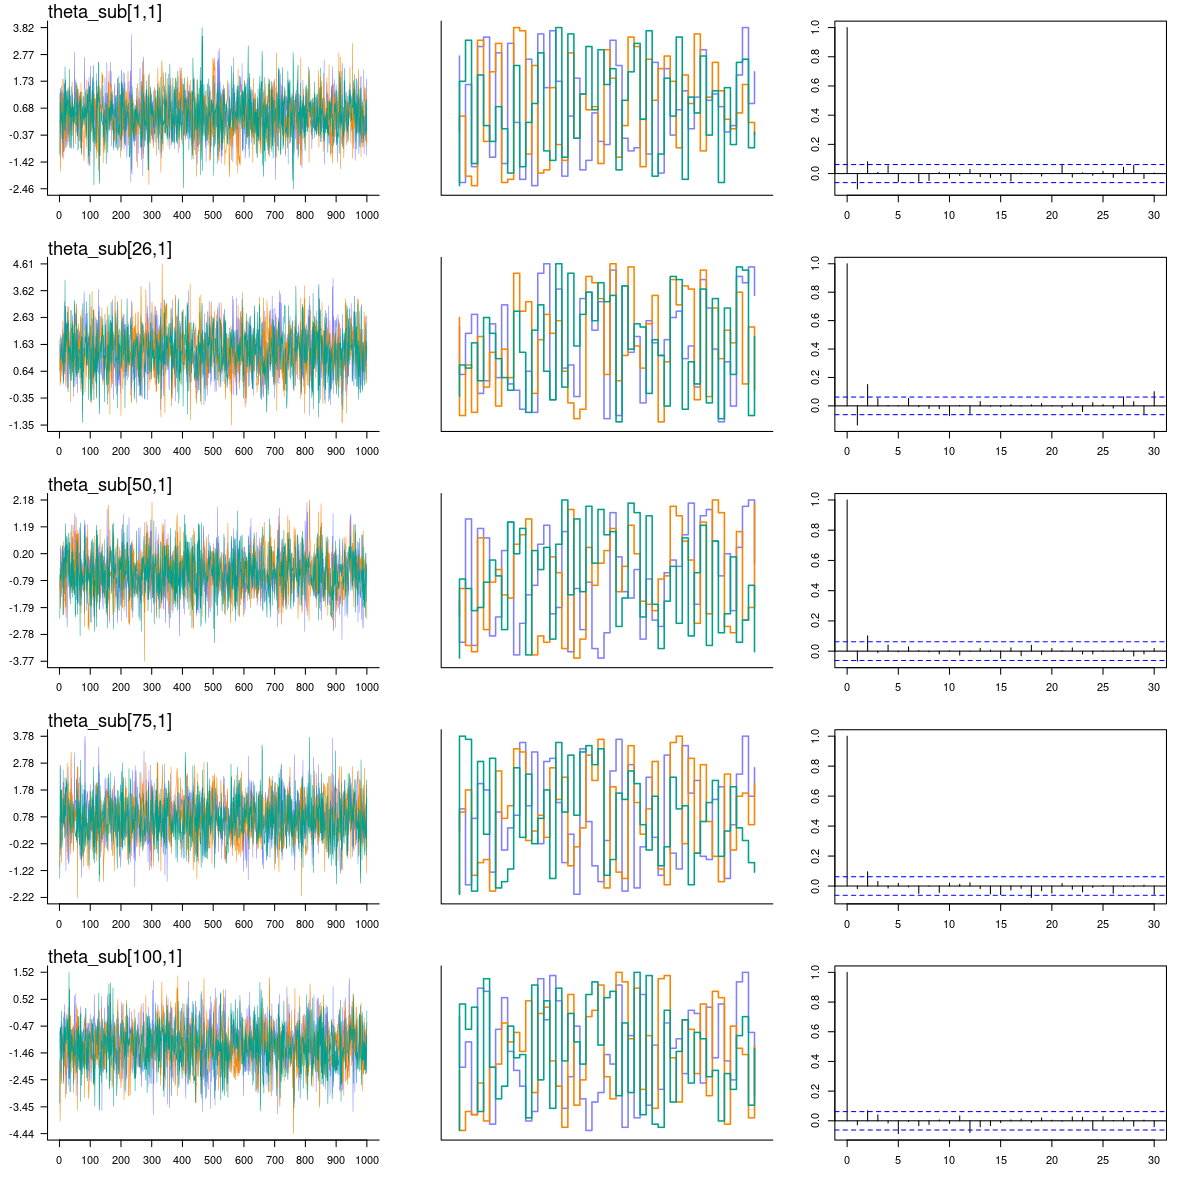
\includegraphics[width=1\linewidth]{FOLV_NC_J100_Ndata6_theta_sub1}
	%
	\caption[First-Order latent variable model (FOLV). Non-centered parametrization. Individual's first sub-dimension. Trace, trank and auto-correlation plots.]%
	{First-Order latent variable model (FOLV). Non-centered parametrization. Individual's first sub-dimension: (Left) trace plot, (Middle) trank plot, (Right) auto-correlation plot.}
	\label{fig:FOLV_NC_chains4}
\end{figure}
%
\begin{figure}[H]
	\centering
	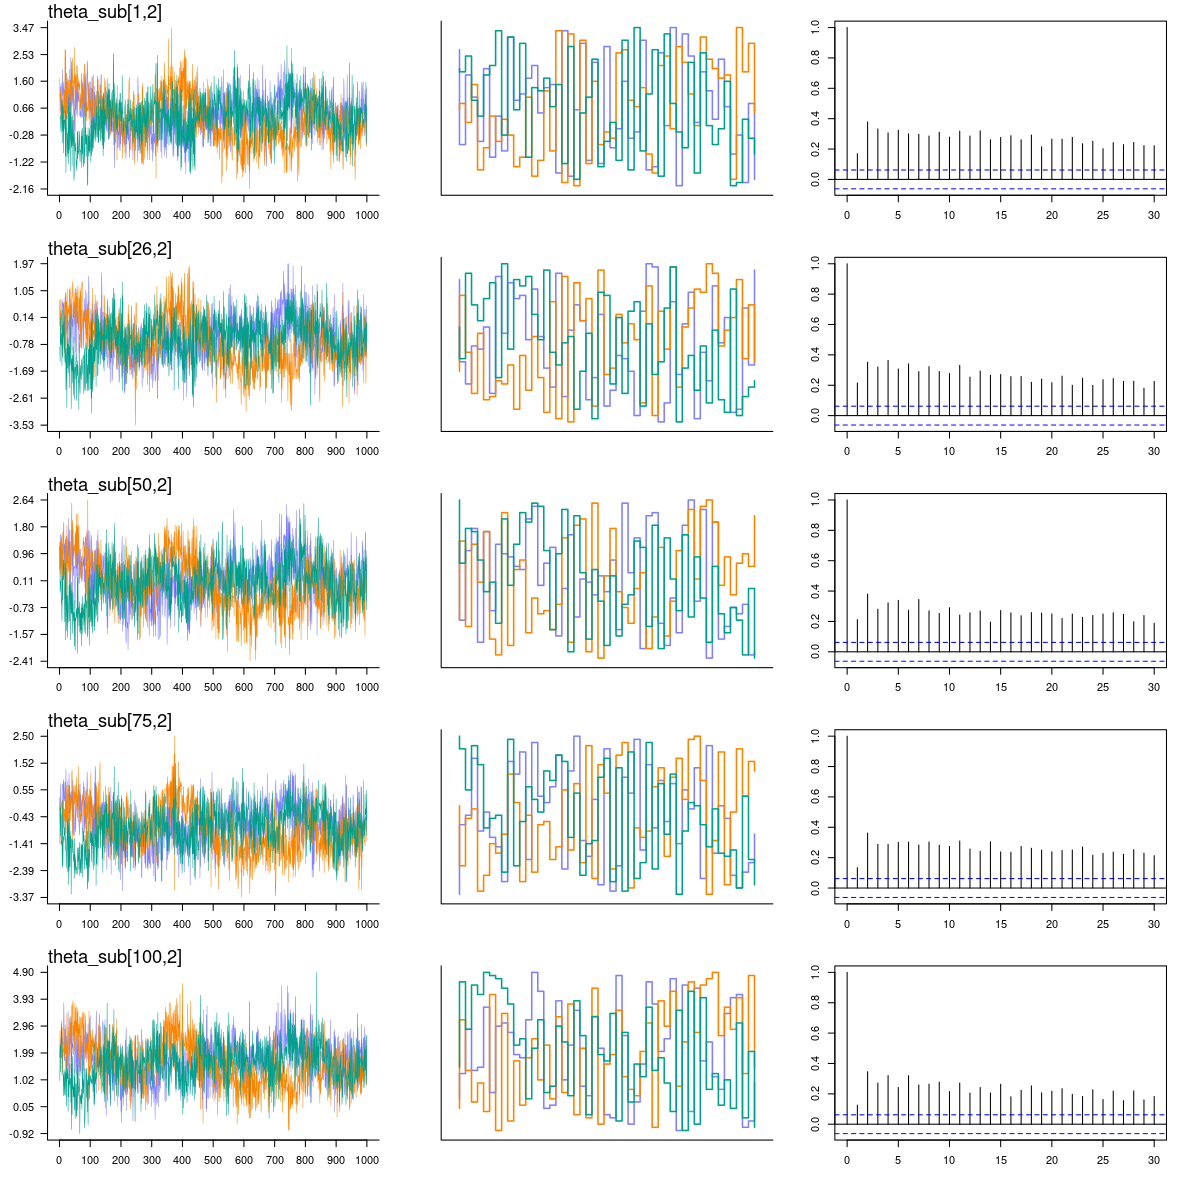
\includegraphics[width=1\linewidth]{FOLV_CE_J100_Ndata7_theta_sub2}
	%
	\caption[First-Order latent variable model (FOLV). Centered parametrization. Individual's second sub-dimension. Trace, trank and auto-correlation plots.]%
	{First-Order latent variable model (FOLV). Centered parametrization. Individual's second sub-dimension: (Left) trace plot, (Middle) trank plot, (Right) auto-correlation plot.}
	\label{fig:FOLV_CE_chains5}
\end{figure}
%
\begin{figure}[H]
	\centering
	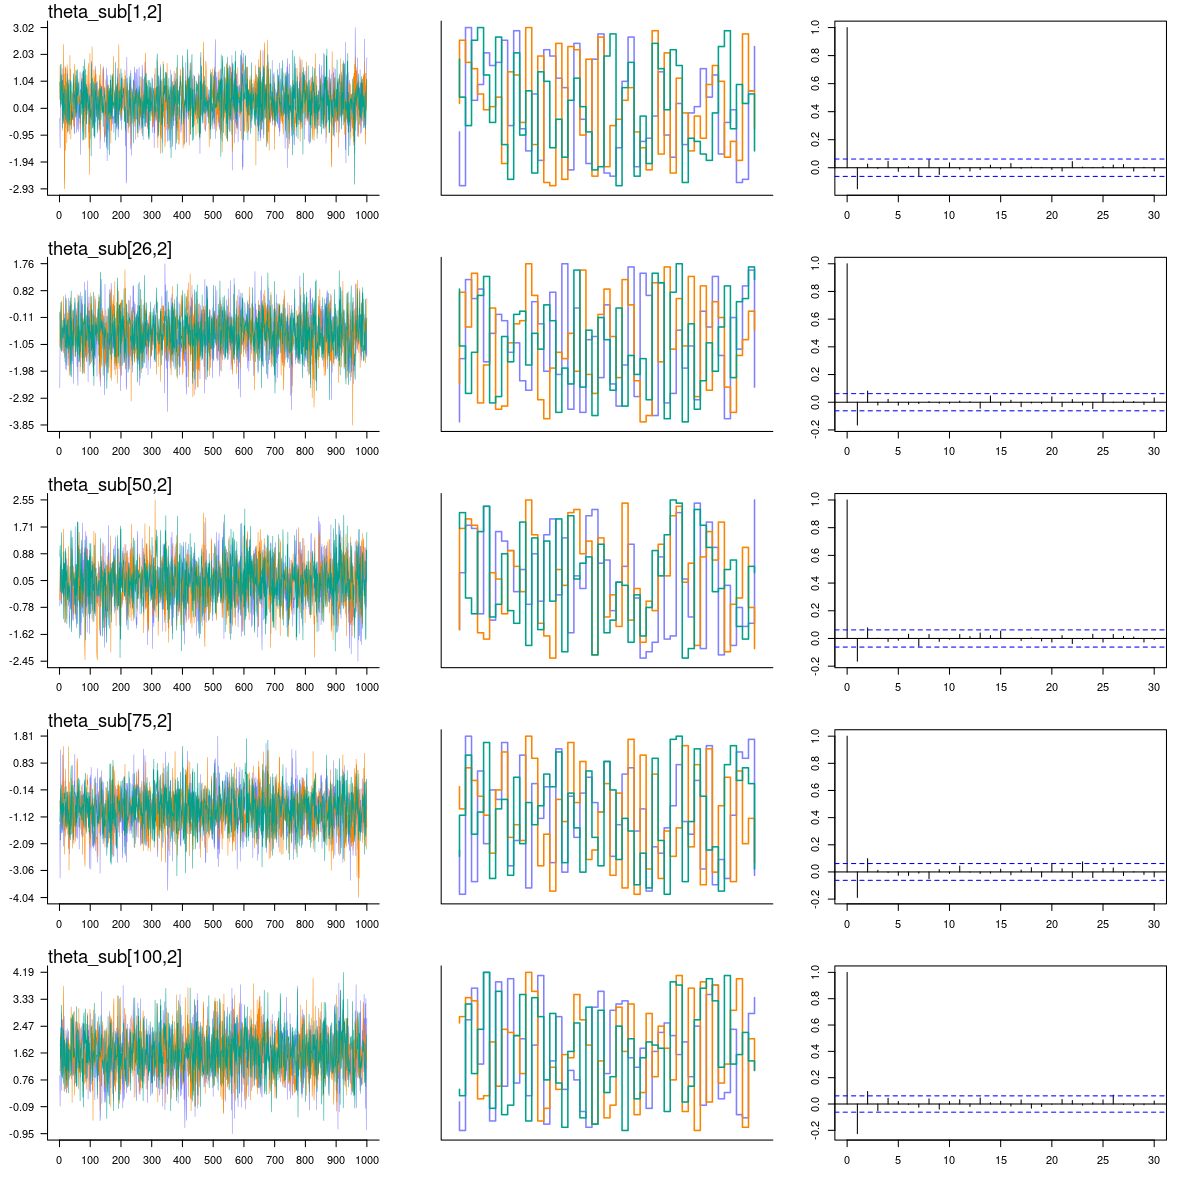
\includegraphics[width=1\linewidth]{FOLV_NC_J100_Ndata7_theta_sub2}
	%
	\caption[First-Order latent variable model (FOLV). Non-centered parametrization. Individual's second sub-dimension. Trace, trank and auto-correlation plots.]%
	{First-Order latent variable model (FOLV). Non-centered parametrization. Individual's second sub-dimension: (Left) trace plot, (Middle) trank plot, (Right) auto-correlation plot.}
	\label{fig:FOLV_NC_chains5}
\end{figure}
%
\begin{figure}[H]
	\centering
	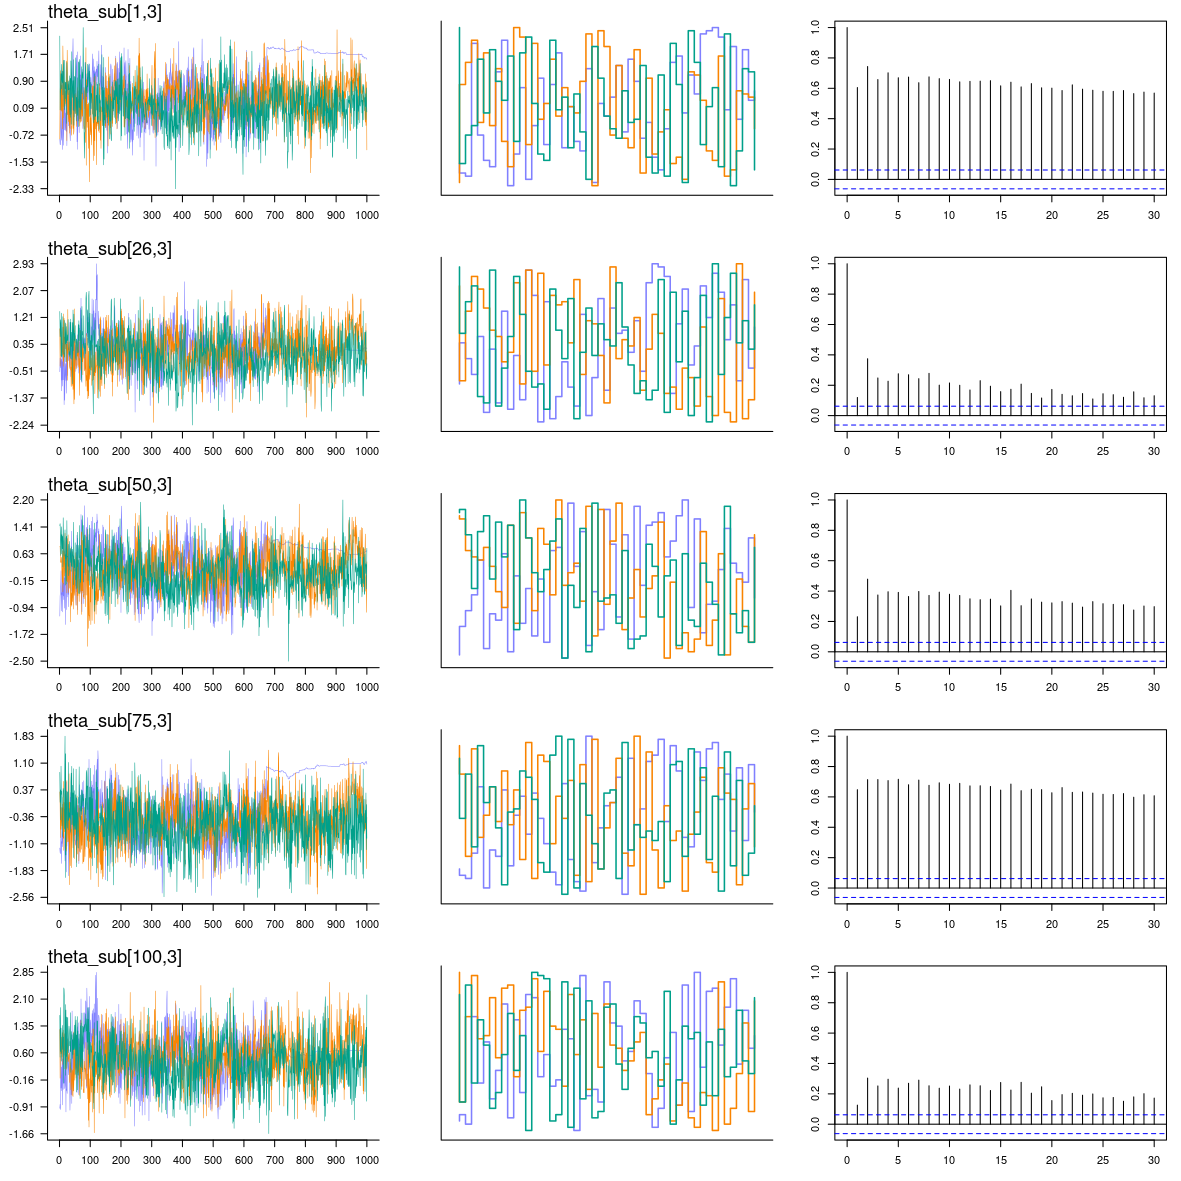
\includegraphics[width=1\linewidth]{FOLV_CE_J100_Ndata8_theta_sub3}
	%
	\caption[First-Order latent variable model (FOLV). Centered parametrization. Individual's third sub-dimension. Trace, trank and auto-correlation plots.]%
	{First-Order latent variable model (FOLV). Centered parametrization. Individual's third sub-dimension: (Left) trace plot, (Middle) trank plot, (Right) auto-correlation plot.}
	\label{fig:FOLV_CE_chains6}
\end{figure}
%
\begin{figure}[H]
	\centering
	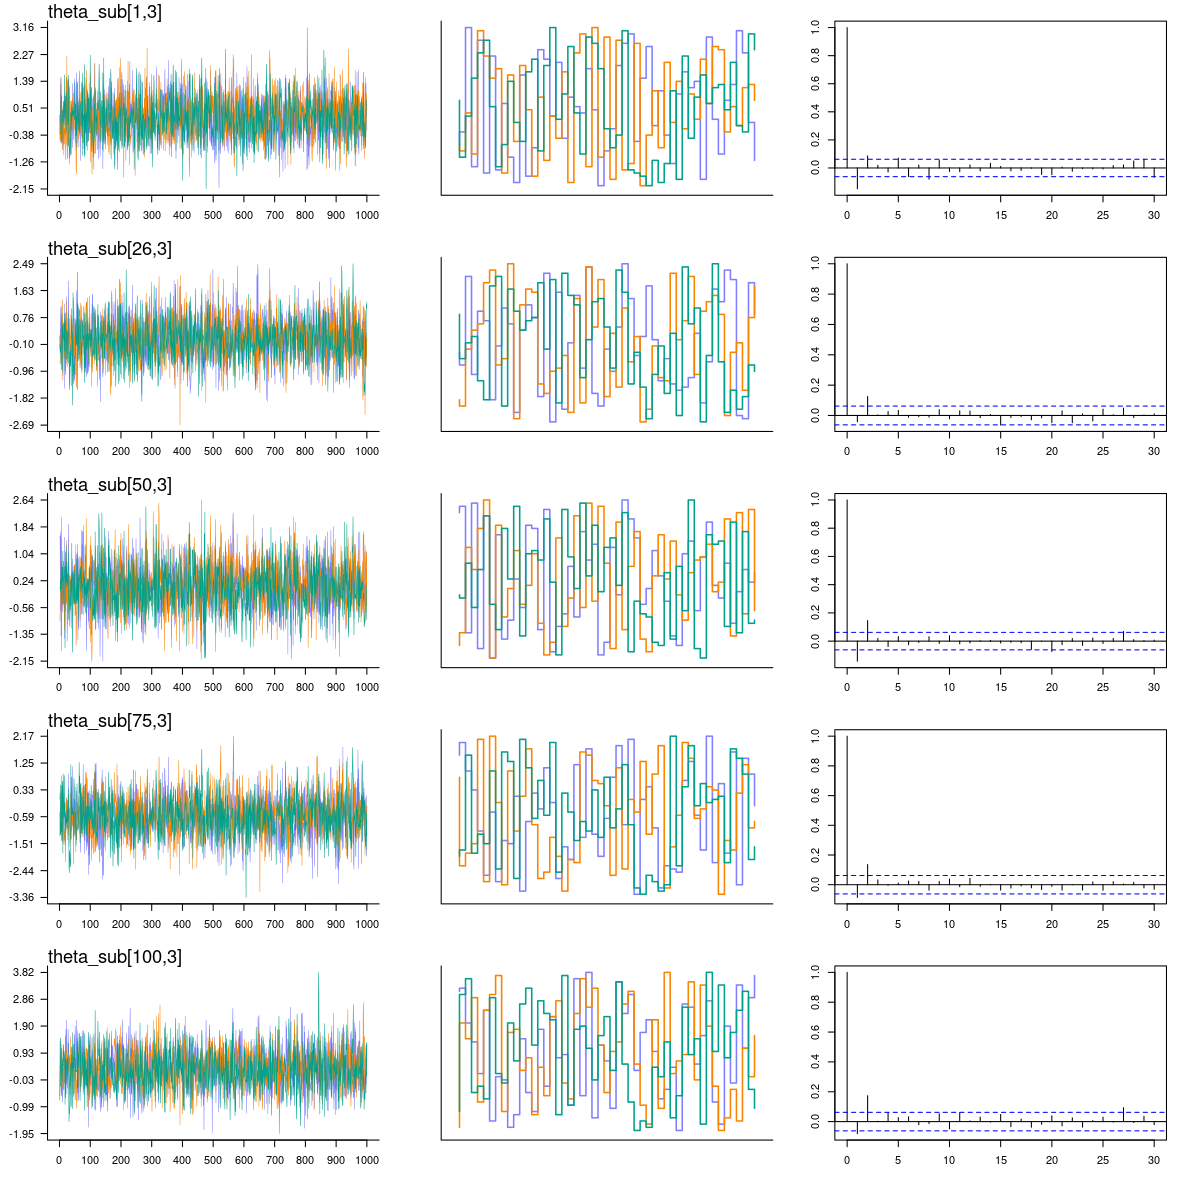
\includegraphics[width=1\linewidth]{FOLV_NC_J100_Ndata8_theta_sub3}
	%
	\caption[First-Order latent variable model (FOLV). Non-centered parametrization. Individual's third sub-dimension. Trace, trank and auto-correlation plots.]%
	{First-Order latent variable model (FOLV). Non-centered parametrization. Individual's third sub-dimension: (Left) trace plot, (Middle) trank plot, (Right) auto-correlation plot.}
	\label{fig:FOLV_NC_chains6}
\end{figure}
%
\begin{figure}[H]
	\centering
	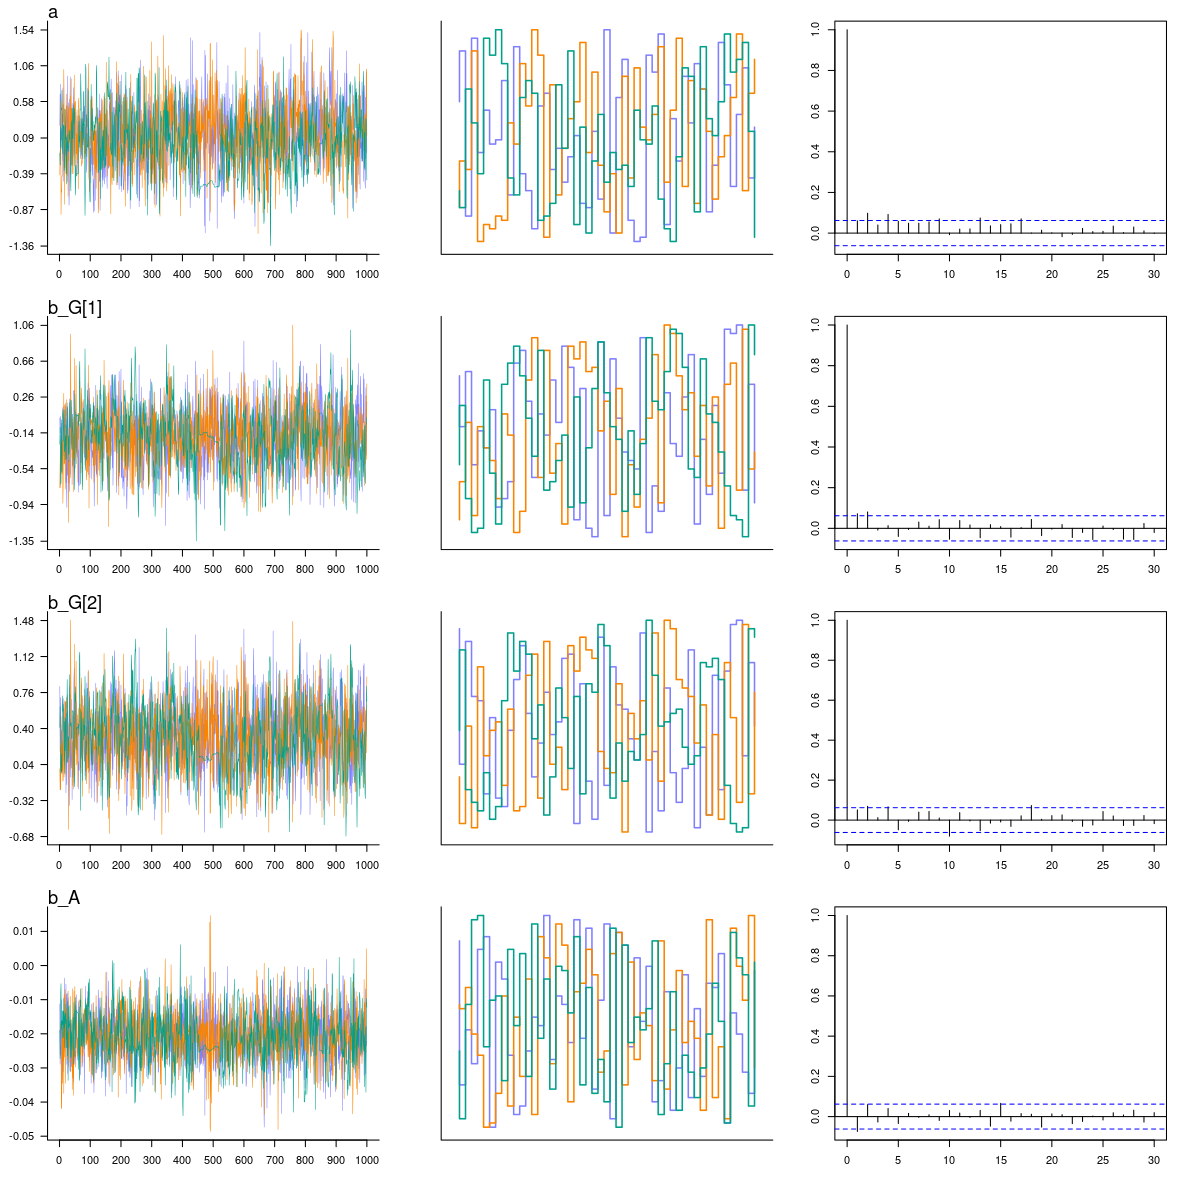
\includegraphics[width=1\linewidth]{FOLV_CE_J100_Ndata4_reg1}
	%
	\caption[First-Order latent variable model (FOLV). Centered parametrization. Regression parameters. Trace, trank and auto-correlation plots.]%
	{First-Order latent variable model (FOLV). Centered parametrization. Regression parameters: (Left) trace plot, (Middle) trank plot, (Right) auto-correlation plot.}
	\label{fig:FOLV_CE_chains7}
\end{figure}
%
\begin{figure}[H]
	\centering
	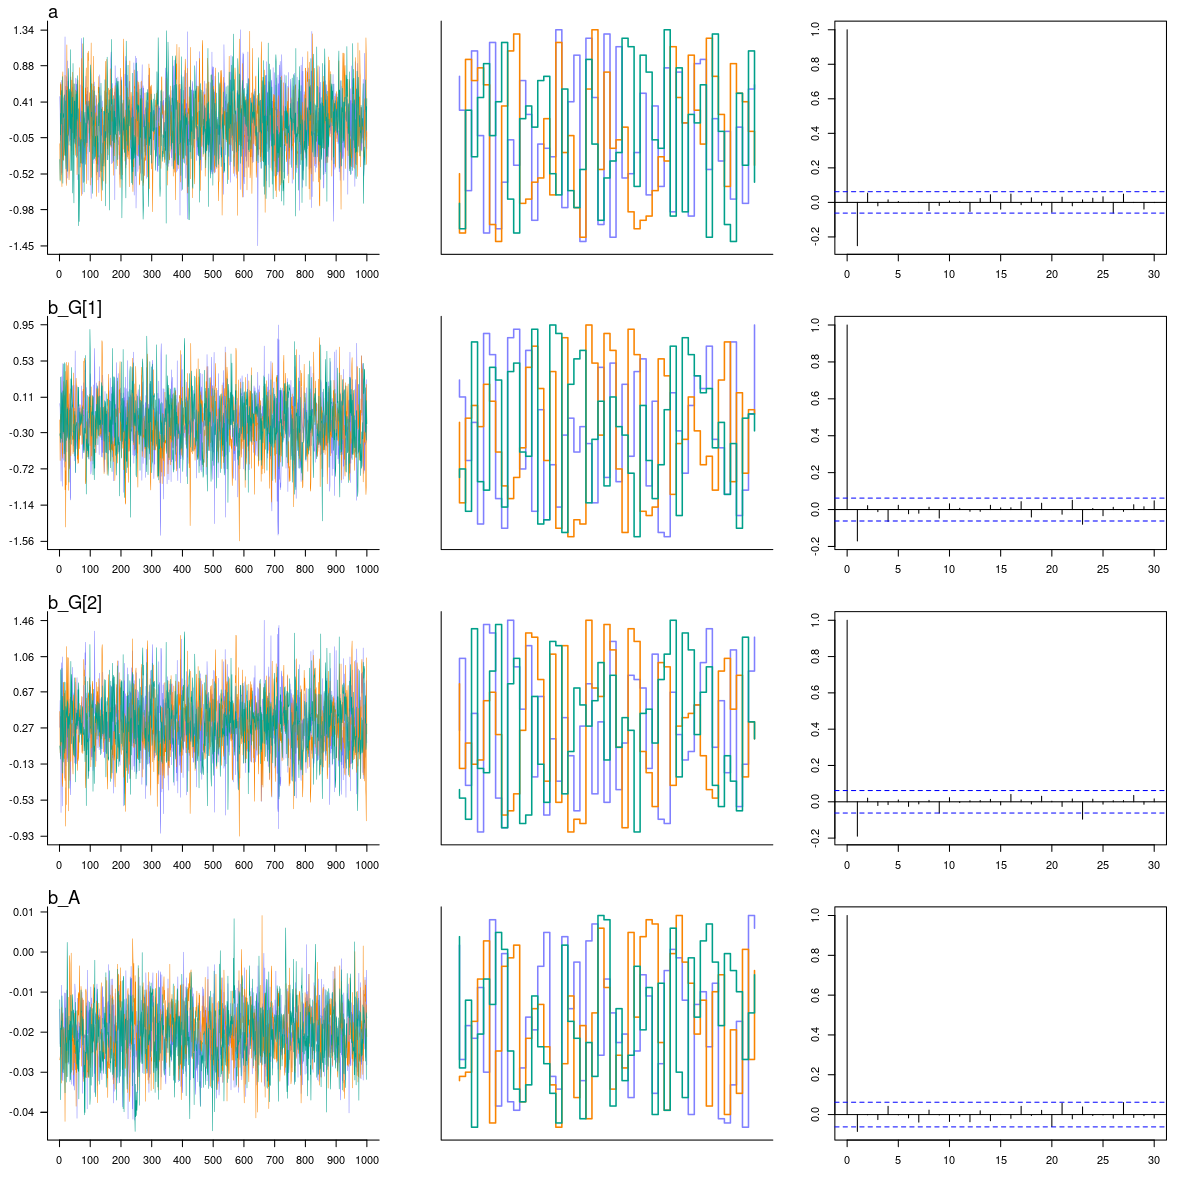
\includegraphics[width=1\linewidth]{FOLV_NC_J100_Ndata4_reg1}
	%
	\caption[First-Order latent variable model (FOLV). Non-centered parametrization. Regression parameters. Trace, trank and auto-correlation plots.]%
	{First-Order latent variable model (FOLV). Non-centered parametrization. Regression parameters: (Left) trace plot, (Middle) trank plot, (Right) auto-correlation plot.}
	\label{fig:FOLV_NC_chains7}
\end{figure}
%
\begin{figure}[H]
	\centering
	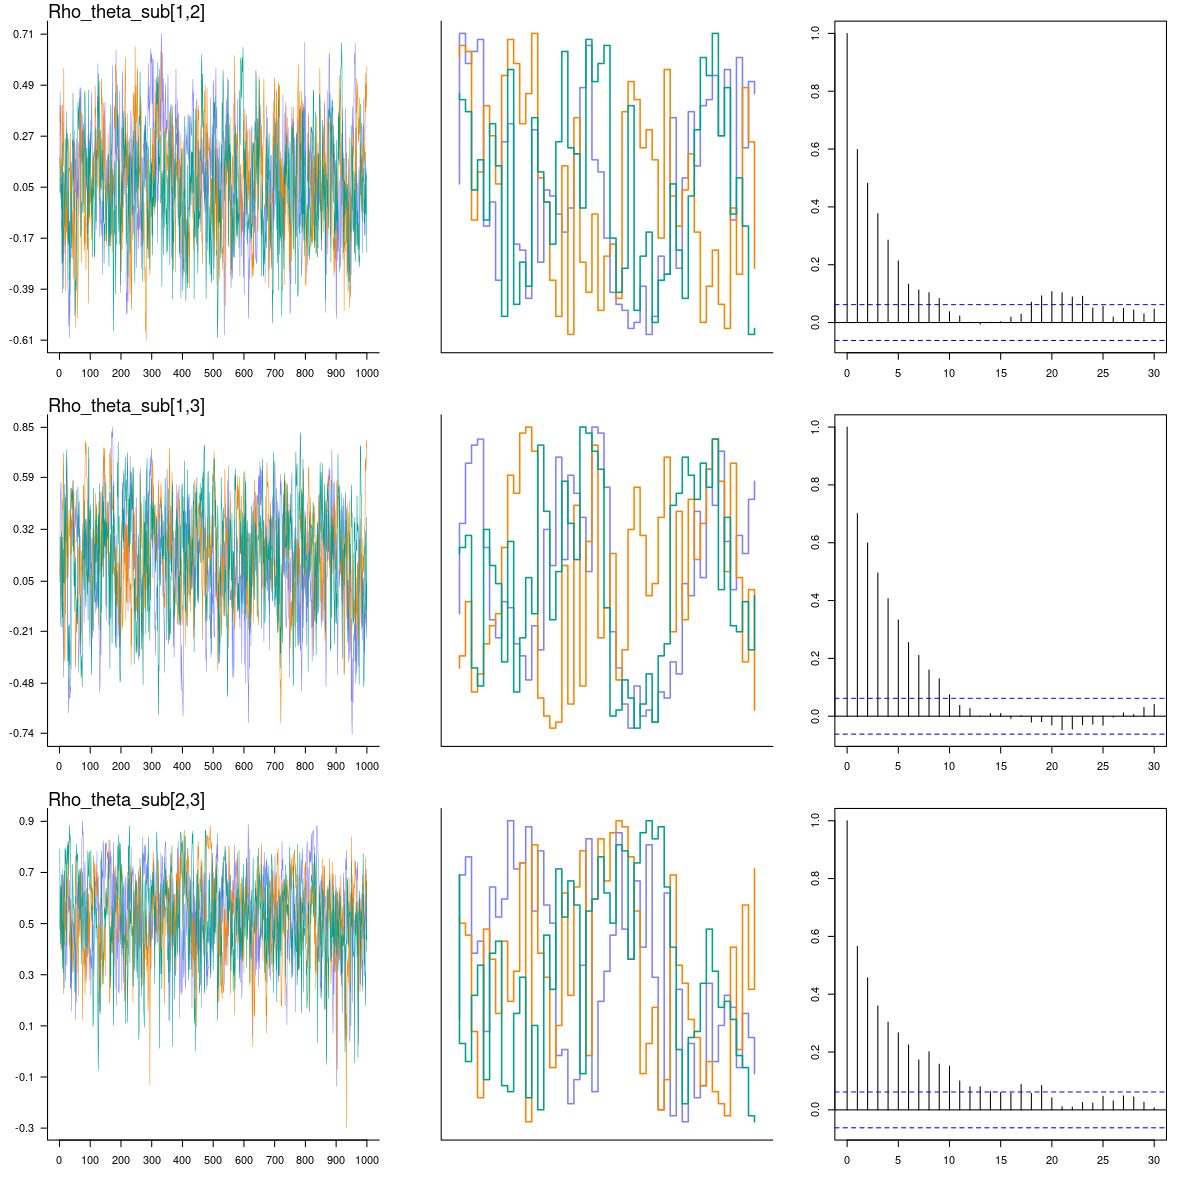
\includegraphics[width=1\linewidth]{FOLV_CE_J100_Ndata5_Rho}
	%
	\caption[First-Order latent variable model (FOLV). Centered parametrization. Correlation of sub-dimensions. Trace, trank and auto-correlation plots.]%
	{First-Order latent variable model (FOLV). Centered parametrization. Correlation of sub-dimensions: (Left) trace plot, (Middle) trank plot, (Right) auto-correlation plot.}
	\label{fig:FOLV_CE_chains8}
\end{figure}
%
\begin{figure}[H]
	\centering
	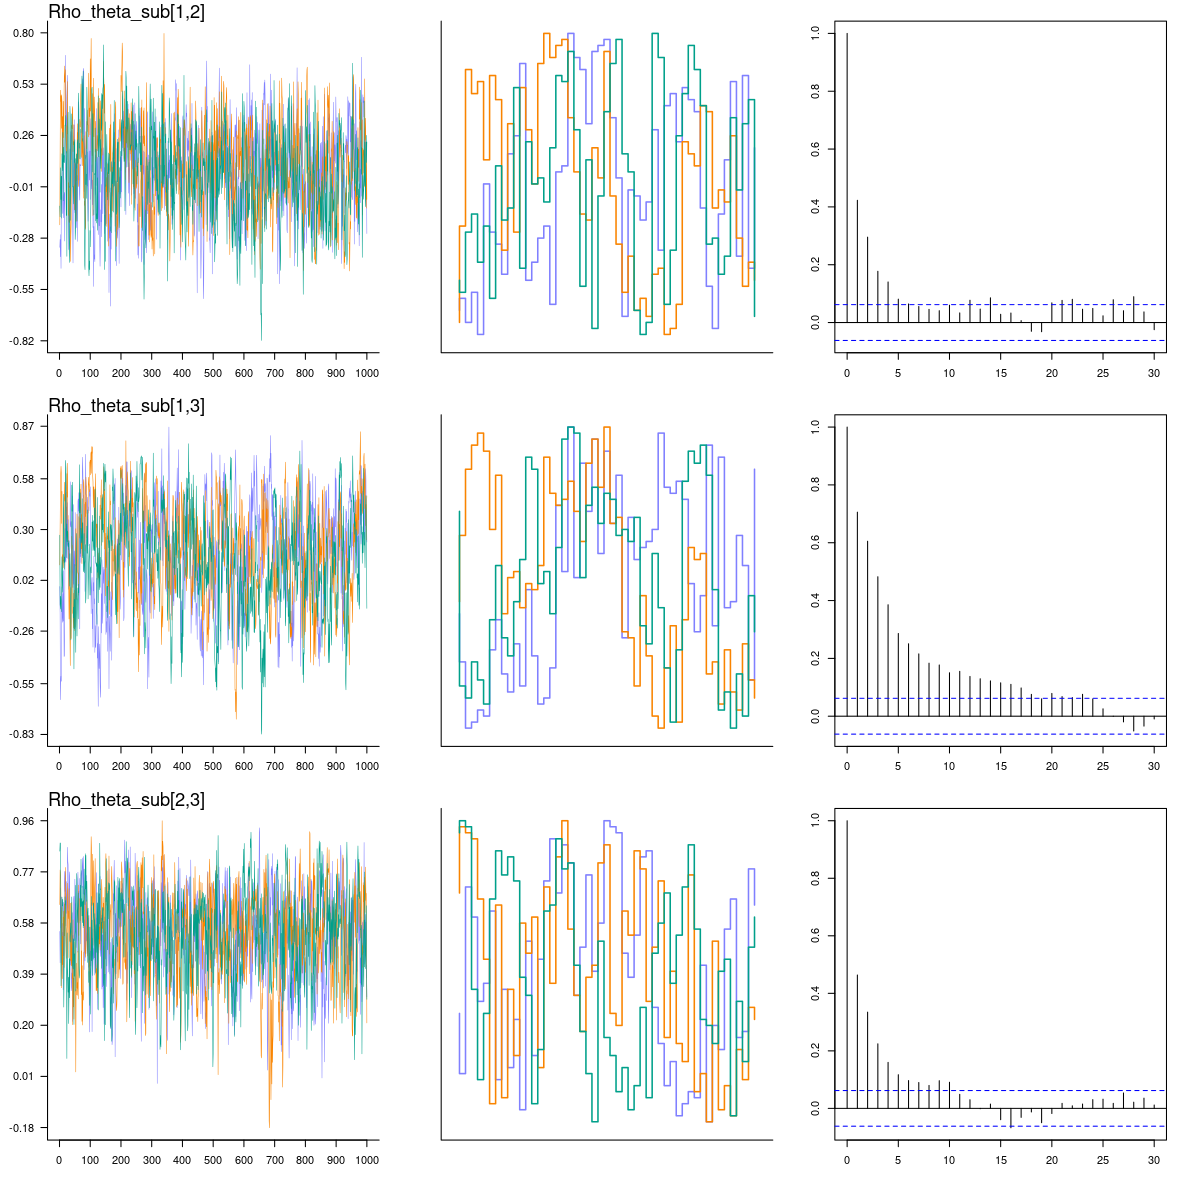
\includegraphics[width=1\linewidth]{FOLV_NC_J100_Ndata5_Rho}
	%
	\caption[First-Order latent variable model (FOLV). Non-centered parametrization. Correlation of sub-dimensions. Trace, trank and auto-correlation plots.]%
	{First-Order latent variable model (FOLV). Non-centered parametrization. Correlation of sub-dimensions: (Left) trace plot, (Middle) trank plot, (Right) auto-correlation plot.}
	\label{fig:FOLV_NC_chains8}
\end{figure}
%
\begin{figure}[H]
	\centering
	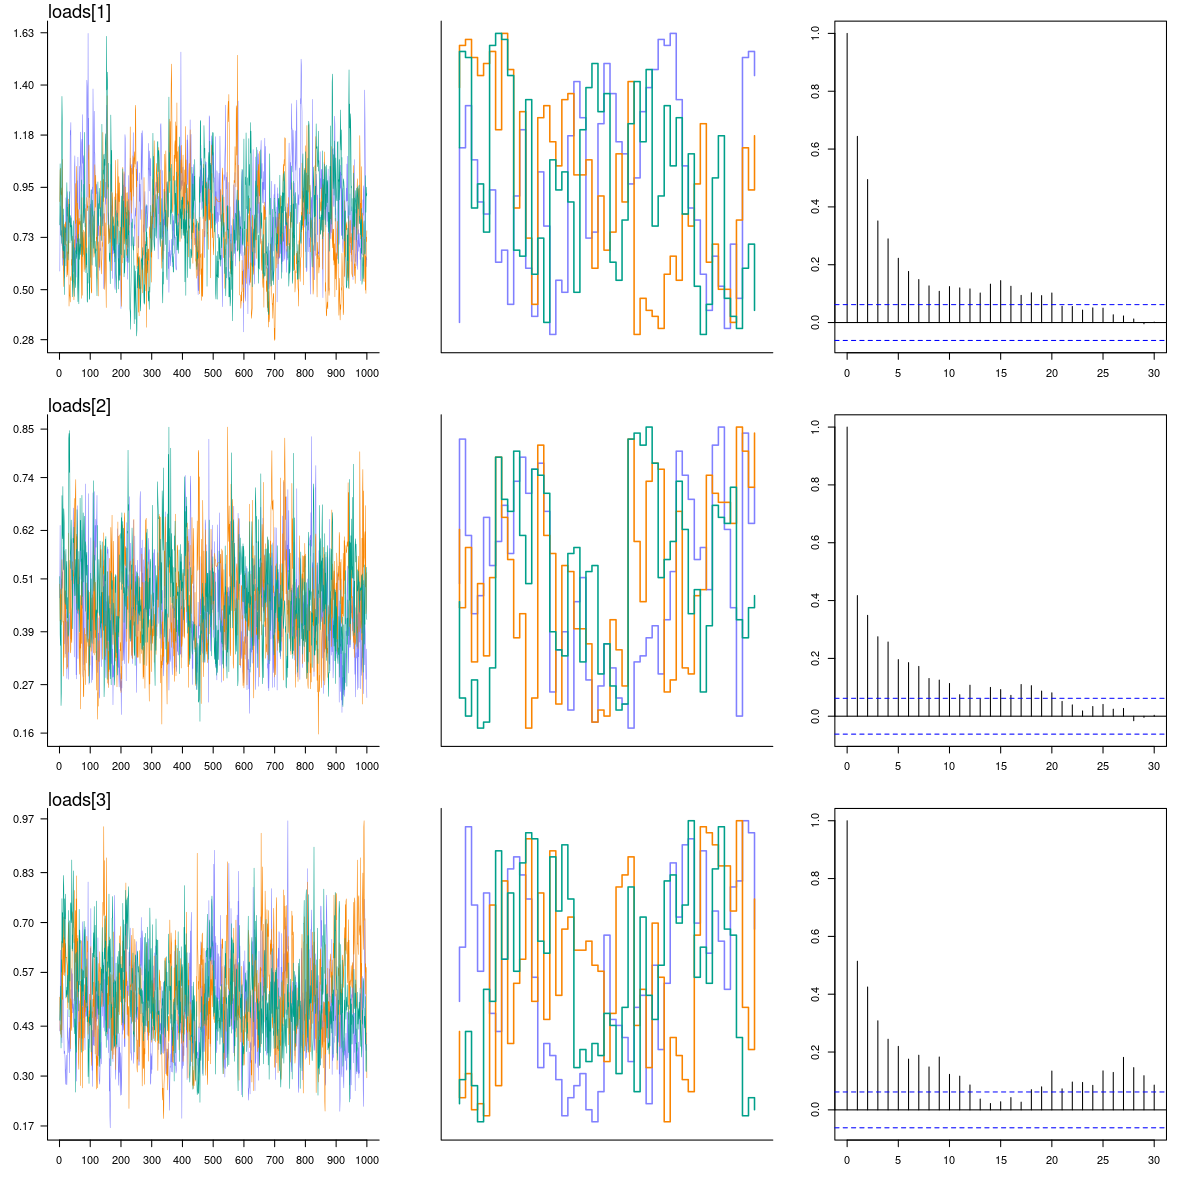
\includegraphics[width=1\linewidth]{SOLV_CE_J100_Ndata9_loads}
	%
	\caption[Second-Order latent variable model (SOLV). Centered parametrization. Loadings. Trace, trank and auto-correlation plots.]%
	{Second-Order latent variable model (SOLV). Centered parametrization. Loadings: (Left) trace plot, (Middle) trank plot, (Right) auto-correlation plot.}
	\label{fig:SOLV_CE_chains1}
\end{figure}
%
\begin{figure}[H]
	\centering
	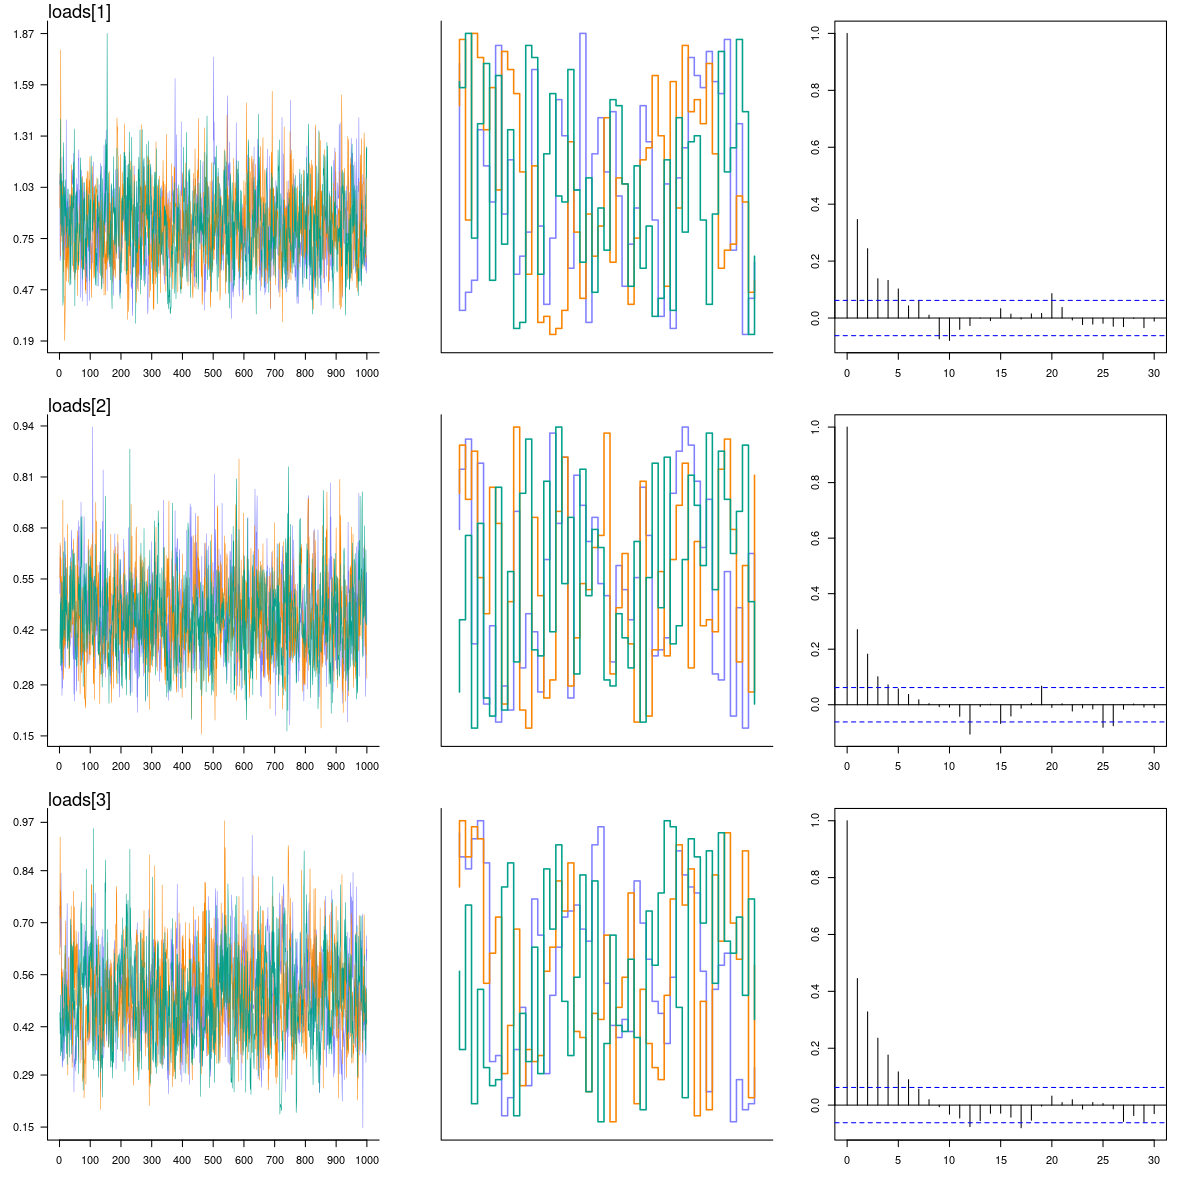
\includegraphics[width=1\linewidth]{SOLV_NC_J100_Ndata9_loads}
	%
	\caption[Second-Order latent variable model (SOLV). Non-centered parametrization. Loadings. Trace, trank and auto-correlation plots.]%
	{Second-Order latent variable model (SOLV). Non-centered parametrization. Loadings: (Left) trace plot, (Middle) trank plot, (Right) auto-correlation plot.}
	\label{fig:SOLV_NC_chains1}
\end{figure}
%
\begin{figure}[H]
	\centering
	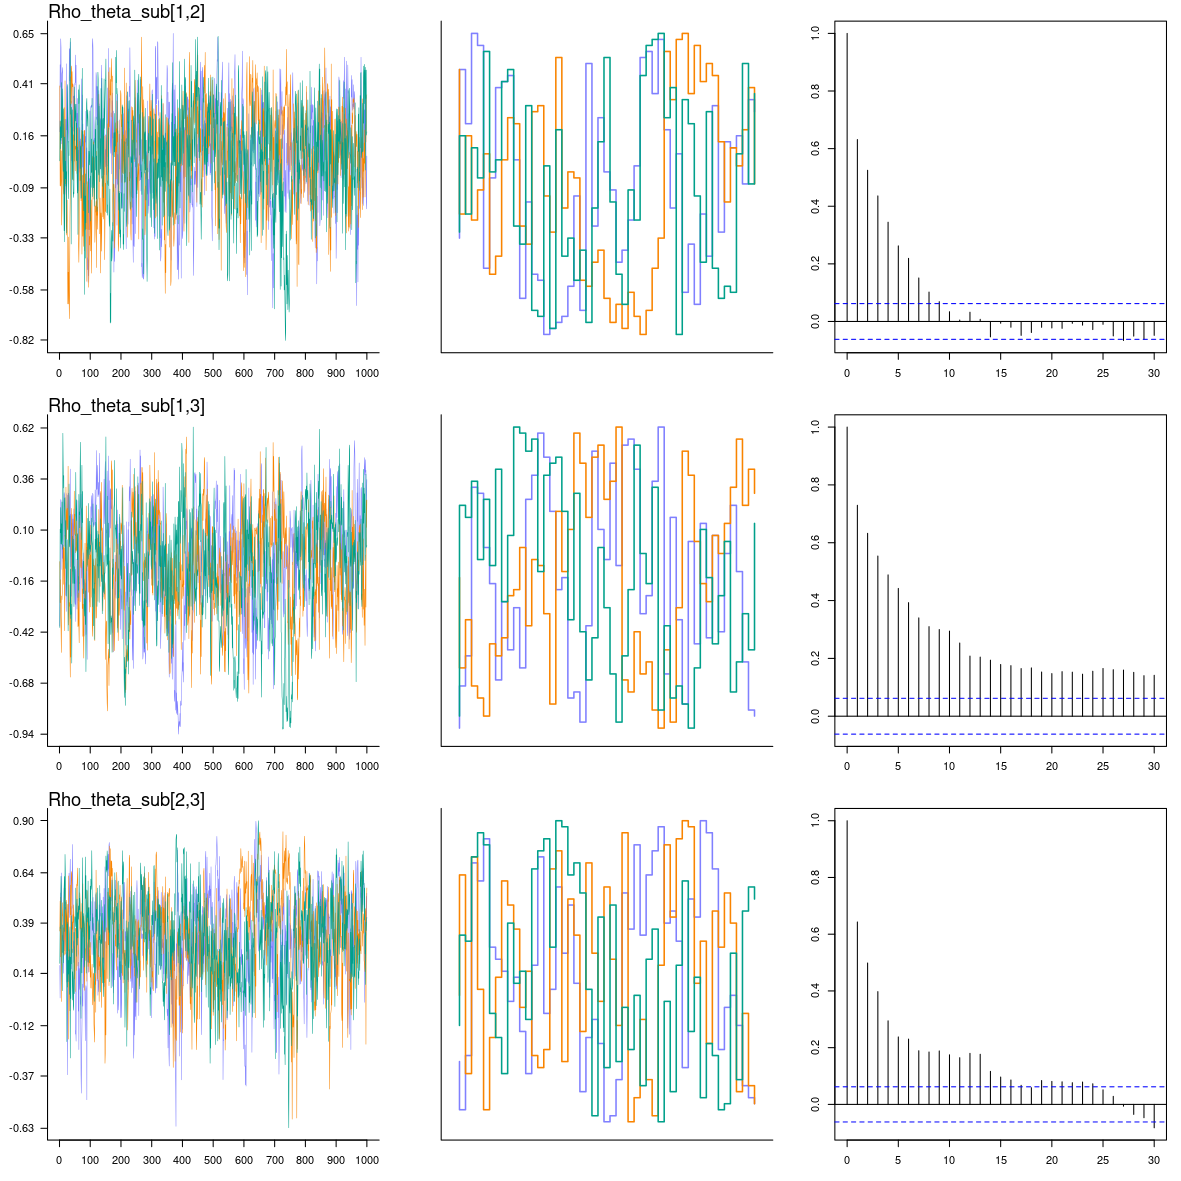
\includegraphics[width=1\linewidth]{SOLV_CE_J100_Ndata1_Rho}
	%
	\caption[Second-Order latent variable model (SOLV). Centered parametrization. Correlation of sub-dimensions. Trace, trank and auto-correlation plots.]%
	{Second-Order latent variable model (SOLV). Centered parametrization. Correlation of sub-dimensions: (Left) trace plot, (Middle) trank plot, (Right) auto-correlation plot.}
	\label{fig:SOLV_CE_chains2}
\end{figure}
%
\begin{figure}[H]
	\centering
	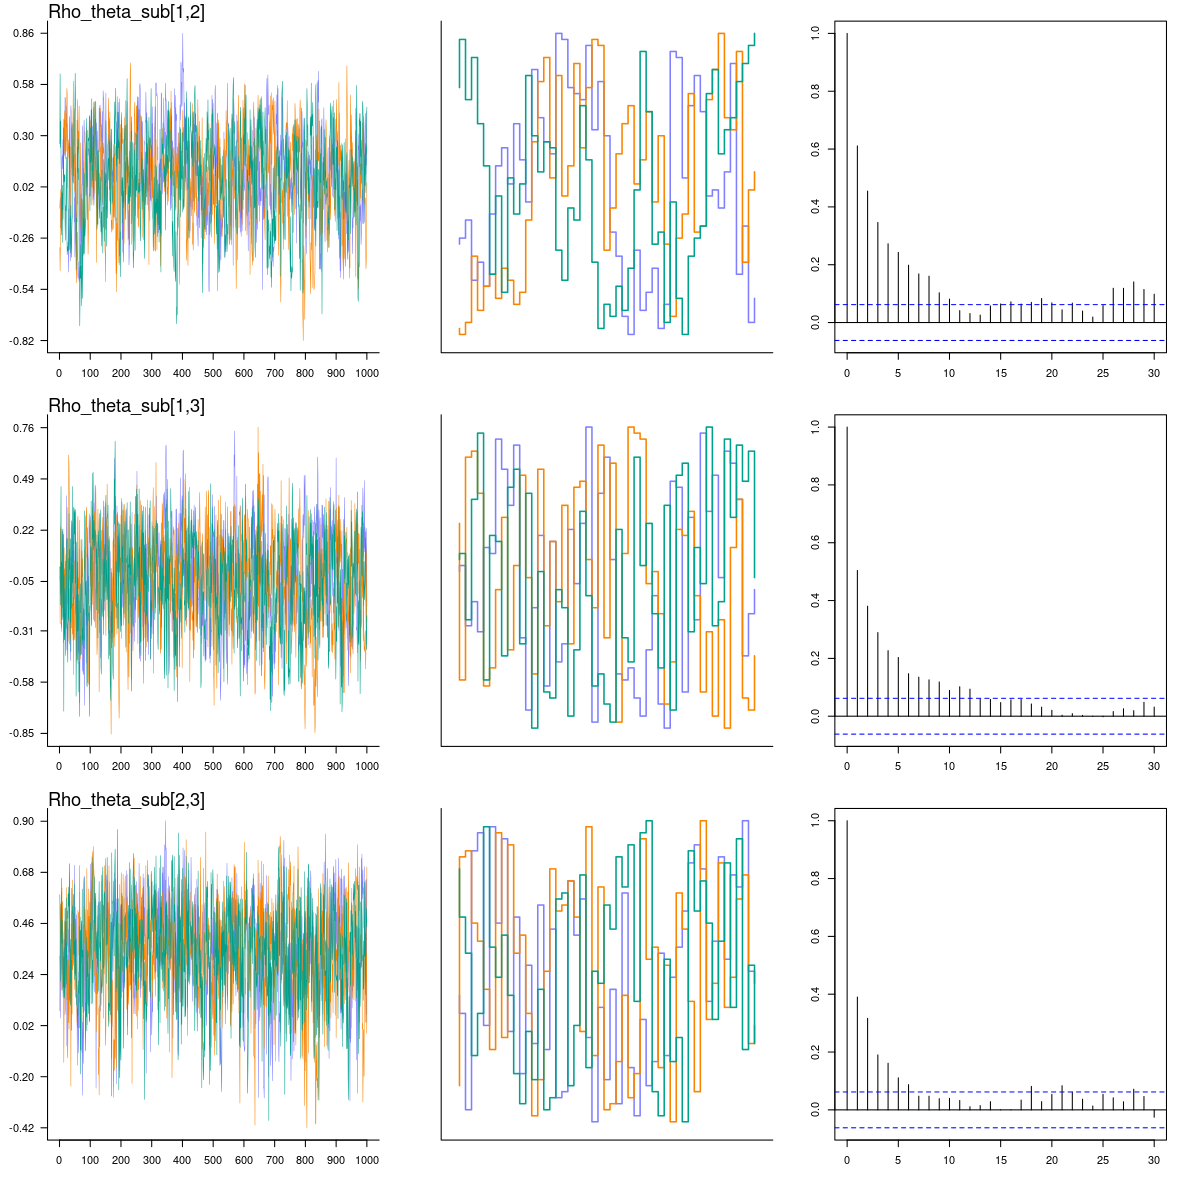
\includegraphics[width=1\linewidth]{SOLV_NC_J100_Ndata1_Rho}
	%
	\caption[Second-Order latent variable model (SOLV). Non-centered parametrization. Correlation of sub-dimensions. Trace, trank and auto-correlation plots.]%
	{Second-Order latent variable model (SOLV). Non-centered parametrization. Correlation of sub-dimensions: (Left) trace plot, (Middle) trank plot, (Right) auto-correlation plot.}
	\label{fig:SOLV_NC_chains2}
\end{figure}
%
\begin{figure}[H]
	\centering
	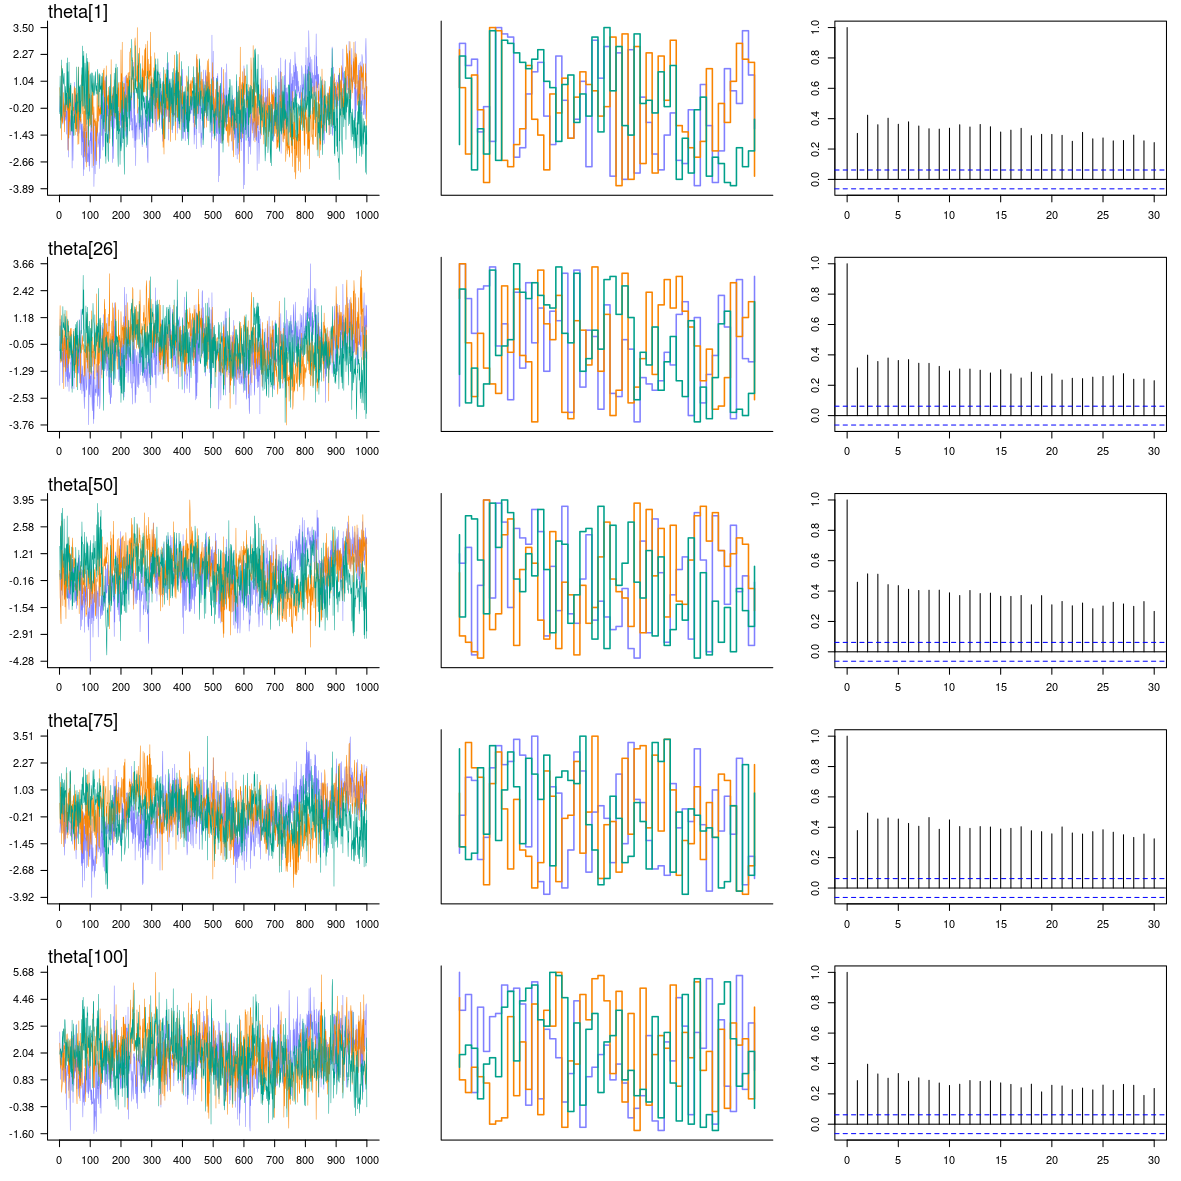
\includegraphics[width=1\linewidth]{SOLV_CE_J100_Ndata10_theta}
	%
	\caption[Second-Order latent variable model (SOLV). Centered parametrization. Highest-order dimension. Trace, trank and auto-correlation plots.]%
	{Second-Order latent variable model (SOLV). Centered parametrization. Highest-order dimension: (Left) trace plot, (Middle) trank plot, (Right) auto-correlation plot.}
	\label{fig:SOLV_CE_chains3}
\end{figure}
%
\begin{figure}[H]
	\centering
	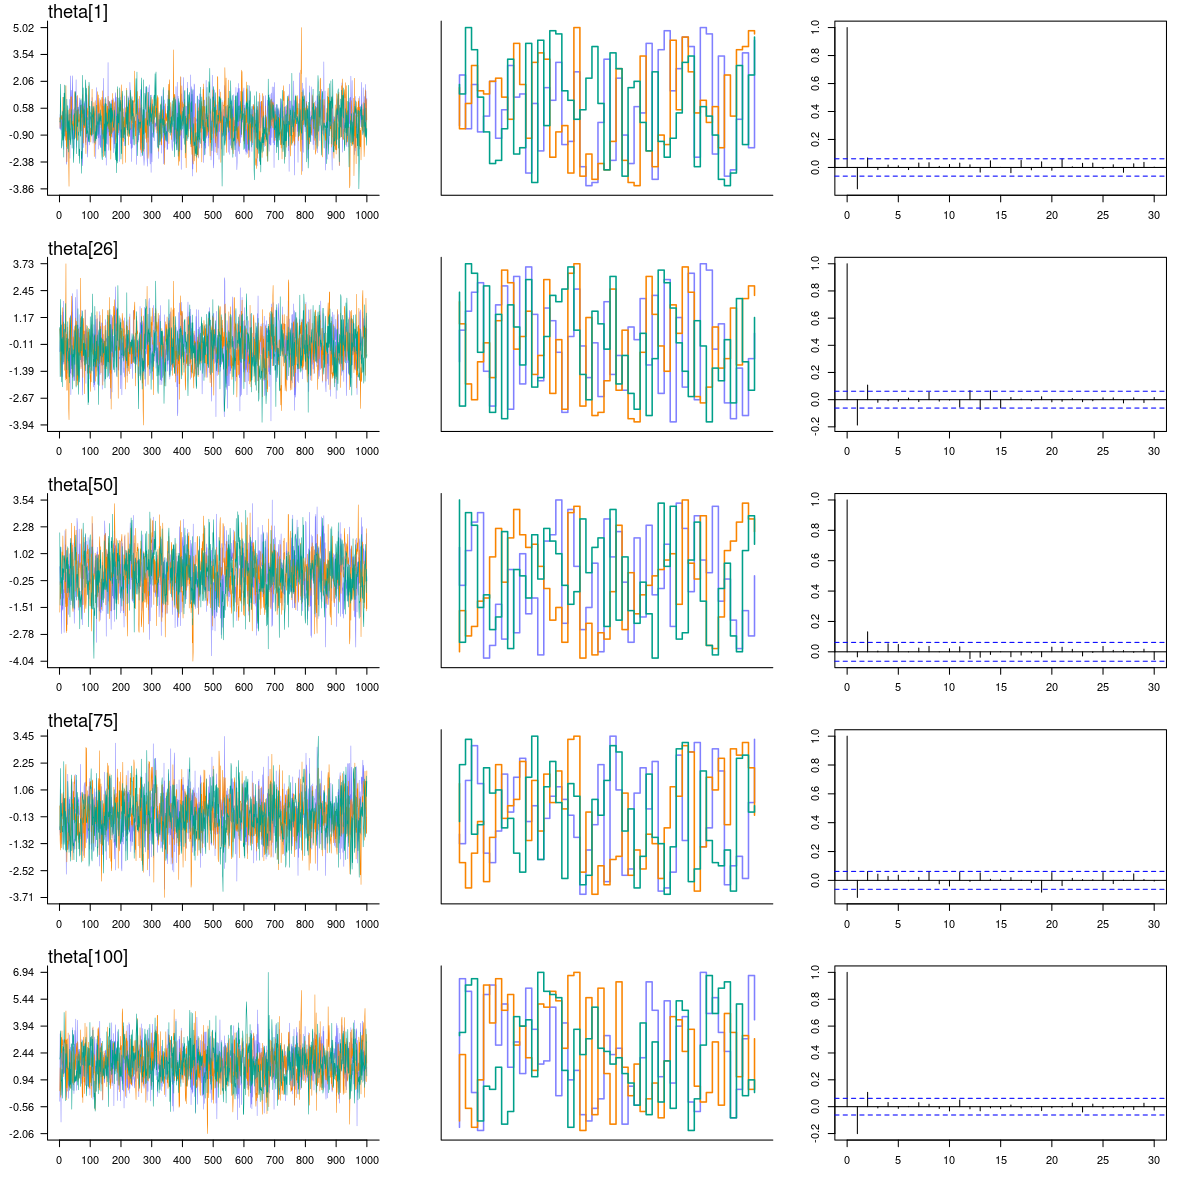
\includegraphics[width=1\linewidth]{SOLV_NC_J100_Ndata10_theta}
	%
	\caption[Second-Order latent variable model (SOLV). Non-centered parametrization. Highest-order dimension. Trace, trank and auto-correlation plots.]%
	{Second-Order latent variable model (SOLV). Non-centered parametrization. Highest-order dimension: (Left) trace plot, (Middle) trank plot, (Right) auto-correlation plot.}
	\label{fig:SOLV_NC_chains3}
\end{figure}
\chapter{Code} \label{appC:additional}

%%%%%%%%%%%%%%%%%%%%%%%%%%%%%%%%%%%%%%%%%%%%%%%%%%%%%%%%%%%%%%%%%%%%%%%
%%%%%%%%%%%%%%%%%%%%%%%%%%%%%%%%%%%%%%%%%%%%%%%%%%%%%%%%%%%%%%%%%%%%%%%

\section{Chapter 3: Bayesian estimation} \label{appC1:chapter3}

\subsection{To center or not to center} \label{appC1_1:noncenter}

\subsubsection{The devil's funnel, centered parametrization.} 

\noindent \textbf{Stan}
%
\begin{lstlisting}[language=R]
transformed data {
	int<lower=0> J;
	J = 1;
}
parameters {
	real theta[J];
	real v;
}
model {
	v ~ normal(0, 3);
	theta ~ normal(0, exp(v));
}
\end{lstlisting}


\noindent \textbf{JAGS}
%
\begin{lstlisting}[language=R]
model{
	v ~ dnorm(0,3)
	theta ~ dnorm(0, exp(v))
}
\end{lstlisting}



%%%%%%%%%%%%%%%%%%%%%%%%%%%%%%%%%%%%%%%%%%%%%%%%%%%%%%%%%%%%%%%%%%%%%%%

\subsubsection{The devil's funnel, centered parametrization with priors.} 

\noindent \textbf{Stan}
%
\begin{lstlisting}[language=R]
transformed data {
	int<lower=0> J;
	J = 1;
}
parameters {
	real theta[J];
	real v;
}
model {
	v ~ normal(0, 1);
	theta ~ normal(0, exp(v));
}
\end{lstlisting}


\noindent \textbf{JAGS}
%
\begin{lstlisting}[language=R]
model{
	v ~ dnorm(0,1)
	theta ~ dnorm(0, exp(v))
}
\end{lstlisting}


%%%%%%%%%%%%%%%%%%%%%%%%%%%%%%%%%%%%%%%%%%%%%%%%%%%%%%%%%%%%%%%%%%%%%%%

\subsubsection{The devil's funnel, non-centered parametrization.}

\noindent \textbf{Stan}
%
\begin{lstlisting}[language=R]
transformed data {
	int<lower=0> J;
	J = 1;
}
parameters {
	real ztheta[J];
	real v;
}
transformed parameters{
	vector[J] theta;
	theta = exp(v) * to_vector( ztheta );
}
model {
	v ~ normal(0, 3);
	ztheta ~ normal(0, 1);
}
\end{lstlisting}


\noindent \textbf{JAGS}
%
\begin{lstlisting}[language=R]
model{
	v ~ dnorm(0,1)
	ztheta ~ dnorm(0,1)
	theta = v * ztheta
}
\end{lstlisting}


%%%%%%%%%%%%%%%%%%%%%%%%%%%%%%%%%%%%%%%%%%%%%%%%%%%%%%%%%%%%%%%%%%%%%%%
%%%%%%%%%%%%%%%%%%%%%%%%%%%%%%%%%%%%%%%%%%%%%%%%%%%%%%%%%%%%%%%%%%%%%%%


\section{Chapter 4: Simulation study} \label{appC2:chapter4}

\subsection{Algorithm} \label{appC2_1:sim}

\noindent \textbf{Data generation}
%
\begin{lstlisting}[language=R]
S = 10 # ten data sets
condition = expand_grid( J = c(100, 250, 500), load=0.95)
for(i in 1:nrow(condition)){
	for(s in 1:S){
		with(condition[i,],
			data_generation( J=J, loads=rep(load, 3), 
				Ndata=s, seed=4587+s+i, # different seeds
				file_dir=file.path(getwd(), 'data') ) )
	}
}
\end{lstlisting}

\noindent \textbf{Data generation function}
%
\begin{lstlisting}[language=R]
# function:
#     data_generation
# description:  
#     To generate data based on different parameter settings.
#     Only two parameters are effectively controlled in the experimentation: 
#     sample size (J), and the loading from the SOLV to the FOLV (loads).
# characteristics of the sample design:
#   - one instrument
#   - hierarchical measurement scales with FOLV and SOLV
#   - one evaluation time
#   - one sample of individuals
#   - testlet items, multiple items come from one text
#   - with covariates
#   - NO missingness
# arguments:
#     J = individual sample sizes
#     loads = loadings from SOLV to FOLV (it control correlation)
#     Ndata = defines the number of data generated
#     file_dir = path to save generated data
#     s_theta = sd to simulate SOLV and FOLV
#     s_text = sd in generating items from a specific text
#     D = number of dimensions (default 3)
#     K = number of items (default 25)
#     L = number of texts (default 5), it has to be a multiple of K
#     seed = seed used to generate the simulation (default 1)
#     prec = rounding in abilities and item parameters (default 3)
	
data_generation =function( J=100, loads=rep(0.95, 3), Ndata=1, file_dir,
	s_theta=0.5, s_text=0.5, D=3, K=25, L=5, seed=1, prec=3){
		
#_______________
# 1. generation 
#_______________
set.seed(seed)
		
	
## 1.1. regression parameters
mom = expand_grid(a=loads[-3], b=loads[-1])
mom = mom[-3,]
		
betas = list( gender = c(0, 0.5),
	age = -0.02,
	edu = c(-0.5, 0.5, 0),
	exp = c(-0.5, 0, 0.35, 0.5),
	loads = loads, # loadings
	exp_corr = with(mom, a*b) ) # expected correlation
		
		
## 1.2 covariates
abilities = data.frame( IDind=1:J,
	gender = sample(c(1,2), size=J, replace=T),
	age = sample(30:65, size=J, replace=T),
	edu = sample(c(1,2,3), size=J, replace=T),
	exp = sample(c(1,2,3,4), size=J, replace=T),
	theta=rep(NA,J), theta1=rep(NA,J), 
	theta2=rep(NA,J), theta3=rep(NA,J) )
	
# variable indices
SOLV_loc = which(names(abilities)=='theta')
FOLV_loc = which(names(abilities)=='theta1'):
	which(names(abilities)==paste0('theta', D))
		
		
## 1.3. abilities
# SOLV
m_theta = rep(NA, J)
for(j in 1:J){
	ageC = with(abilities, age[j] - min(age) + 1 )
	
	m_theta[j] = with(abilities,
		betas$gender[ gender[j] ] + 
		betas$age * ageC +
		betas$edu[ edu[j] ] + 
		betas$exp[ exp[j] ] )  
}
abilities[, SOLV_loc] = round( rnorm(J, m_theta, s_theta), prec)
		
# FOLV
# independent after considering SOLV
s_mult = diag( rep(s_theta, D) ) 
m_mult = data.frame( theta1=rep(NA, J), 
	theta2=rep(NA, J), 
	theta3=rep(NA, J) )
for(j in 1:J){
	m_mult[j,] = betas$loads * abilities$theta[j]
	abilities[j, FOLV_loc] = round( 
		mvrnorm(n=1, mu=unlist(m_mult[j,]), Sigma=s_mult), prec)
}
		

## 1.4 texts
texts = data.frame(IDtext=1:L, m_b=rep(NA, L), s_b=rep(NA, L))
texts$m_b = seq(-1.5, 1.5, length.out=L)
texts$s_b = rep(s_text, L)
		
		
## 1.5 items
items = data.frame(IDitem=1:K, IDtext=rep(NA,K), 
	IDdim=rep(NA,K), b=rep(NA, K))
kl = K/L # items per text
for(k in 1:nrow(texts)){
	items$b[(1:kl) + (k-1)*kl] = with(texts, 
		round( rnorm(kl, m_b[k], s_b[k]), prec ) )
	items$IDtext[(1:kl) + (k-1)*kl] = k
}
		
		
## 1.6 dimensions
items$IDdim = sample(1:3, K, replace=T)
		
#_______________
# 2. storage
#_______________
		
## 2.1 parameters
data_true = list(
	
	seed=seed,
	
	# indices
	J = J,
	D = D, 
	K = K, 
	L = L,
		
	# abilities
	betas = betas,
	abilities = abilities,
		
	# texts and items
	texts = texts,
	items = items)
	
	file_name = paste0('Parameters_J',J,'_l',loads[1],
		'_Ndata',Ndata,'.RData')
	save(data_true, file=file.path(file_dir, file_name) )
		
		
		
## 2.2 long format
data_eval = data.frame(
		
	# individual data
	IDind = rep(abilities$IDind, K),
	gender = rep(abilities$gender, K),
	age = rep(abilities$age, K),
	edu = rep(abilities$edu, K),
	exp = rep(abilities$exp, K),
	theta = rep(abilities$theta, K),
	theta1 = rep(abilities$theta1, K),
	theta2 = rep(abilities$theta2, K),
	theta3 = rep(abilities$theta3, K),
		
	# items
	IDitem = rep(items$IDitem, each=J),
	IDtext = rep(items$IDtext, each=J),
	IDdim = rep(items$IDdim, each=J),
	b = rep(items$b, each=J) )
		
# appropriate ability
data_eval$theta_jkld = NA
for(i in 1:nrow(data_eval) ){
	data_eval$theta_jkld[i] = data_eval[i, FOLV_loc[ data_eval$IDdim[i] ] ]
}
		
# linear predictor, probability, and outcome
data_eval$v_jkld = with(data_eval, theta_jkld - b)
data_eval$p_jkld = inv_logit( data_eval$v )
data_eval$y_jkld = rbinom( nrow(data_eval), 1, prob=data_eval$p)
		
file_name = paste0('LongFormat_J',J,'_l',loads[1],
	'_Ndata',Ndata,'.RData')
save(data_eval, file=file.path(file_dir, file_name) )
		
	
## 2.3 estimation data
data_post = list(
		
	# evaluation data
	N = nrow(data_eval),
	J = J,
	K = K,
	L = L,
	D = D,
	IDj = data_eval$IDind,
	IDk = data_eval$IDitem,
	IDl = data_eval$IDtext,
	IDd = data_eval$IDdim,
	GE = data_eval$gender,
	AG = data_eval$age,
	ED = data_eval$edu,
	XP = data_eval$exp,
	y = data_eval$y_jkld,
		
	# individual data
	IDind = abilities$IDind,
	G = abilities$gender,
	A = abilities$age,
	E = abilities$edu,
	X = abilities$exp,
		
	# items
	IDitem = items$IDitem,
	IDtext = items$IDtext,
	IDdim = items$IDdim )
		
file_name = paste0('ListFormat_J',J,'_l',loads[1],
	'_Ndata',Ndata,'.RData')
save(data_post, file=file.path(file_dir, file_name) )
		
}
\end{lstlisting}





%%%%%%%%%%%%%%%%%%%%%%%%%%%%%%%%%%%%%%%%%%%%%%%%%%%%%%%%%%%%%%%%%%%%%%%

\subsection{Results} \label{appC2_2:results}

\subsubsection{Models}

it has the stan model used to analize the data \\

\noindent \textbf{FOLV CP}
%
\begin{lstlisting}[language=R]
data{
	// evaluation
	int N;
	int J;
	int K;
	int L;
	int D;
	int IDj[N];
	int IDk[N];
	int IDl[N];
	int IDd[N];
	int GE[N];
	real AG[N];
	int ED[N];
	int XP[N];
	int y[N];
	
	// individuals
	int IDind[J];
	int G[J];
	real A[J];
	int E[J];
	int X[J];
	
	// items
	int IDitem[K];
	int IDtext[K];
	int IDdim[K];
}
parameters{
	// items
	real m_b[L];
	real<lower=0> s_b[L];
	real b_k[K];
	
	// betas
	real a;
	real b_G[2];
	real b_A;
	real b_E[3];
	real b_X[4];
	
	// abilities
	// sub-dimensions: lit, inf, ref
	corr_matrix[D] Rho_theta_sub; 
	vector[D] theta_sub[J]; 
}
model{
	// declare
	vector[D] m_mult[J];
	real v;
	real p;
	
	// items
	m_b ~ normal(0, 1);
	s_b ~ exponential(2);
	for(k in 1:K){            // priors
		b_k[k] ~ normal( m_b[ IDtext[k] ], s_b[ IDtext[k] ]); 
	}
	
	// abilities
	a ~ normal(0, 0.5);
	b_G ~ normal(0, 0.5);
	b_A ~ normal(0, 0.5);
	b_E ~ normal(0, 1);
	b_X ~ normal(0, 0.5);
	Rho_theta_sub ~ lkj_corr(2);
	for(j in 1:J){
		m_mult[j,] = rep_vector( a + b_G[ G[j] ] +
			b_A * ( A[j] - min(A) ) +
			b_E[ E[j] ] + 
			b_X[ X[j] ], D);
		// using the same predictor for the three latents
	}
	theta_sub ~ multi_normal( m_mult, Rho_theta_sub );
	
	// model
	for( i in 1:N ) {
		v = theta_sub[ IDj[i], IDd[i] ] - b_k[ IDk[i] ];
		p = inv_logit(v);
		y[i] ~ bernoulli(p);
	}
}
//# generated quantities{
//#     vector[N] log_lik;
//#     real v;
//#     real p;
//#     
//#     // likelihood
//#     for( i in 1:N ) {
//#       v = theta_sub[ IDj[i], IDd[i] ] - b_k[ IDk[i] ];
//#       p = inv_logit(v);
//#       log_lik[i] = bernoulli_lpmf( y[i] | p);
//#     }
//# }
\end{lstlisting} 


\noindent \textbf{FOLV NCP}
%
\begin{lstlisting}[language=R]
data{
	// evaluation
	int N;
	int J;
	int K;
	int L;
	int D;
	int IDj[N];
	int IDk[N];
	int IDl[N];
	int IDd[N];
	int GE[N];
	real AG[N];
	int ED[N];
	int XP[N];
	int y[N];
	
	// individuals
	int IDind[J];
	int G[J];
	real A[J];
	int E[J];
	int X[J];
	
	// items
	int IDitem[K];
	int IDtext[K];
	int IDdim[K];
}
parameters{
	// items
	real m_b[L];
	real<lower=0> s_b[L];
	real zb_k[K];
	
	// betas
	real a;
	real b_G[2];
	real b_A;
	real b_E[3];
	real b_X[4];
	
	// abilities
	// sub-dimensions: lit, inf, ref
	cholesky_factor_corr[D] L_Rho_theta_sub; 
	matrix[D, J] ztheta_sub; 
}
transformed parameters{
	real b_k[K];
	matrix[D, D] Rho_theta_sub;
	matrix[J, D] m_mult;
	matrix[J, D] theta_sub;
	
	// items
	for(k in 1:K){
		b_k[k] = m_b[ IDtext[k] ] + s_b[ IDtext[k] ] * zb_k[k]; 
	}
	
	// abilities
	Rho_theta_sub = multiply_lower_tri_self_transpose(L_Rho_theta_sub);
	for(j in 1:J){
		m_mult[j,] = rep_row_vector( a + b_G[ G[j] ] + 
			b_A * (A[j] - min(A) ) +
			b_E[ E[j] ] + 
			b_X[ X[j] ], D);
	}
	theta_sub = (L_Rho_theta_sub * ztheta_sub)';
	theta_sub = theta_sub + m_mult;
}
model{
	// declare
	real v;
	real p;
	
	// items
	m_b ~ normal(0, 1);
	s_b ~ exponential(2);
	zb_k ~ normal(0, 1);
	
	// abilities
	a ~ normal(0, 0.5);
	b_G ~ normal(0, 0.5);
	b_A ~ normal(0, 0.5);
	b_E ~ normal(0, 1);
	b_X ~ normal(0, 0.5);
	L_Rho_theta_sub ~ lkj_corr_cholesky(2);
	to_vector(ztheta_sub) ~ normal(0,1);
	
	// model
	for( i in 1:N ) {
		v = theta_sub[ IDj[i], IDd[i] ] - b_k[ IDk[i] ];
		p = inv_logit(v);
		y[i] ~ bernoulli(p);
	}
}
//# generated quantities{
//#     vector[N] log_lik;
//#     real v;
//#     real p;
//#     
//#     // likelihood
//#     for( i in 1:N ) {
//#       v = theta_sub[ IDj[i], IDd[i] ] - b_k[ IDk[i] ];
//#       p = inv_logit(v);
//#       log_lik[i] = bernoulli_lpmf( y[i] | p);
//#     }
//# }
\end{lstlisting}



\noindent \textbf{SOLV CP}
%
\begin{lstlisting}[language=R]
data{
	// evaluation
	int N;
	int J;
	int K;
	int L;
	int D;
	int IDj[N];
	int IDk[N];
	int IDl[N];
	int IDd[N];
	int GE[N];
	real AG[N];
	int ED[N];
	int XP[N];
	int y[N];
	
	// individuals
	int IDind[J];
	int G[J];
	real A[J];
	int E[J];
	int X[J];
	
	// items
	int IDitem[K];
	int IDtext[K];
	int IDdim[K];
}
parameters{
	// items
	real m_b[L];
	real<lower=0> s_b[L];
	real b_k[K];
	
	// betas
	real a;
	real b_G[2];
	real b_A;
	real b_E[3];
	real b_X[4];
	
	// abilities
	vector[J] theta;              // reading comprehension
	real<lower=0> loads[D];       // loadings
	corr_matrix[D] Rho_theta_sub; // sub-dimensions: lit, inf, ref
	vector[D] theta_sub[J]; 
}
model{
	// declare
	vector[J] m_theta;
	vector[D] m_mult[J];
	real v;
	real p;
	
	// items
	m_b ~ normal(0, 1);
	s_b ~ exponential(2);
	for(k in 1:K){            // priors
		b_k[k] ~ normal( m_b[ IDtext[k] ], s_b[ IDtext[k] ]); 
	}
	
	// SOLV
	a ~ normal(0, 0.5);
	b_G ~ normal(0, 0.5);
	b_A ~ normal(0, 0.5);
	b_E ~ normal(0, 1);
	b_X ~ normal(0, 0.5);
	for(j in 1:J){
		m_theta[j] = a + b_G[ G[j] ] + 
			b_A * ( A[j] - min(A) ) +
			b_E[ E[j] ] + 
			b_X[ X[j] ];
	}
	theta ~ normal(m_theta, 1); 
	// setting the scale at this level
	
	// FOLV
	loads ~ lognormal(0, 0.5);
	for(j in 1:J){
		m_mult[j,] = [ loads[1]*theta[j], 
			loads[2]*theta[j], 
			loads[3]*theta[j] ]';
	}
	Rho_theta_sub ~ lkj_corr(2);
	theta_sub ~ multi_normal( m_mult, Rho_theta_sub ); 
	// also setting scale here
	
	// model
	for( i in 1:N ) {
		v = theta_sub[ IDj[i], IDd[i] ] - b_k[ IDk[i] ];
		p = inv_logit(v);
		y[i] ~ bernoulli(p);
	}
}
//# generated quantities{
//#     vector[N] log_lik;
//#     real v;
//#     real p;
//#     
//#     // likelihood
//#     for( i in 1:N ) {
//#       v = theta_sub[ IDj[i], IDd[i] ] - b_k[ IDk[i] ];
//#       p = inv_logit(v);
//#       log_lik[i] = bernoulli_lpmf( y[i] | p);
//#     }
//# }
\end{lstlisting}


\noindent \textbf{SOLV NCP}
%
\begin{lstlisting}[language=R]
data{
	// evaluation
	int N;
	int J;
	int K;
	int L;
	int D;
	int IDj[N];
	int IDk[N];
	int IDl[N];
	int IDd[N];
	int GE[N];
	real AG[N];
	int ED[N];
	int XP[N];
	int y[N];
	
	// individuals
	int IDind[J];
	int G[J];
	real A[J];
	int E[J];
	int X[J];
	
	// items
	int IDitem[K];
	int IDtext[K];
	int IDdim[K];
}
parameters{
	// items
	real m_b[L];
	real<lower=0> s_b[L];
	real zb_k[K];
	
	// betas
	real a;
	real b_G[2];
	real b_A;
	real b_E[3];
	real b_X[4];
	
	// abilities
	vector[J] ztheta;             // reading comprehension
	real<lower=0> loads[D];       // loadings
	cholesky_factor_corr[D] L_Rho_theta_sub; // sub-dimensions
	matrix[D, J] ztheta_sub; 
}
transformed parameters{
	real b_k[K];
	vector[J] m_theta;
	vector[J] theta;             // reading comprehension
	matrix[D, D] Rho_theta_sub;
	matrix[J, D] m_mult;
	matrix[J, D] theta_sub;
	
	// items
	for(k in 1:K){
		b_k[k] = m_b[ IDtext[k] ] + s_b[ IDtext[k] ] * zb_k[k]; 
	}
	
	// SOLV
	for(j in 1:J){
		m_theta[j] = a + b_G[ G[j] ] + 
		b_A * ( A[j] - min(A) ) +
		b_E[ E[j] ] + 
		b_X[ X[j] ];
	}
	theta = m_theta + 1 * ztheta;
	// setting the scale at this level
	
	// FOLV
	Rho_theta_sub = multiply_lower_tri_self_transpose(L_Rho_theta_sub);
	for(j in 1:J){
		m_mult[j,] = to_row_vector( [ loads[1]*theta[j], 
		loads[2]*theta[j], 
		loads[3]*theta[j] ] );
	}
	theta_sub = m_mult + (L_Rho_theta_sub * ztheta_sub)';
	// also setting scale here
}
model{
	// declare
	real v;
	real p;
	
	// items
	m_b ~ normal(0, 1);
	s_b ~ exponential(2);
	zb_k ~ normal(0, 1);
	
	// abilities
	a ~ normal(0, 0.5);
	b_G ~ normal(0, 0.5);
	b_A ~ normal(0, 0.5);
	b_E ~ normal(0, 1);
	b_X ~ normal(0, 0.5);
	ztheta ~ normal(0,1);
	L_Rho_theta_sub ~ lkj_corr_cholesky(2);
	loads ~ lognormal(0, 0.5);
	to_vector(ztheta_sub) ~ normal(0,1);
	
	// model
	for( i in 1:N ) {
		v = theta_sub[ IDj[i], IDd[i] ] - b_k[ IDk[i] ];
		p = inv_logit(v);
		y[i] ~ bernoulli(p);
	}
}
//# generated quantities{
//#     vector[N] log_lik;
//#     real v;
//#     real p;
//#     
//#     // likelihood
//#     for( i in 1:N ) {
//#       v = theta_sub[ IDj[i], IDd[i] ] - b_k[ IDk[i] ];
//#       p = inv_logit(v);
//#       log_lik[i] = bernoulli_lpmf( y[i] | p);
//#     }
//# }
\end{lstlisting}


\subsubsection{Prior predictive investigation}

\noindent \textbf{Prior predictive}
%
\begin{lstlisting}[language=R]
model_path = file.path(getwd(), 'models_prior')
model_list = list.files( model_path )
model_list = model_list[ str_detect(model_list, '.stan') ]

run_prior( models = model_list,
model_path = model_path,
model_out = file.path(getwd(), 'chains_prior'),
data_path = file.path(getwd(), 'data') )
\end{lstlisting}


\noindent \textbf{Prior predictive function}
%
\begin{lstlisting}[language=R]
# function:
#     run_prior
# description:  
#     To run each prior simulation for each model
# arguments:
#     models = list of model to run located in model_path
#     model_path = path where all models are located
#     model_out = path where chains have to be saved
#     data_path = path where data per condition is located

run_prior = function(models, model_path, model_out, data_path){
	
# data list
data_list = list.files( data_path )
data_list = data_list[str_detect(data_list, 'ListFormat')]
	
for(j in 1:length(models) ){
		
	# compile model
	set_cmdstan_path('~/cmdstan')
	mod = cmdstan_model( file.path(model_path, models[j] ) )
	
	# generate base name
	base_nam = str_replace( data_list[1], 'ListFormat_', 
	str_replace( models[j], '.stan', '_') )
	base_nam = str_replace( base_nam, '.RData', '' )
		
	# load data
	load( file.path(data_path, data_list[1] ) )
		
	# run model
	mod$sample(data = data_post, 
		output_dir = model_out, 
		output_basename = base_nam,
		chains=1, parallel_chains=1, adapt_delta=0.99)
	}
}
\end{lstlisting}


\subsubsection{Posterior predictive}

\noindent \textbf{Posterior predictive}
%
\begin{lstlisting}[language=R]
model_path = file.path(getwd(), 'models_post')
model_list = list.files( model_path )
model_list = model_list[ str_detect(model_list, '.stan') ]
model_list = model_list[c(1:2,5:6,3:4)]

run_post( models = model_list,
model_path = model_path,
model_out = file.path(getwd(), 'chains_post'),
data_path = file.path(getwd(), 'data') )
\end{lstlisting}


\noindent \textbf{Posterior predictive function}
%
\begin{lstlisting}[language=R]
# function:
#     run_post
# description:  
#     To run each model for each data in all conditions
# arguments:
#     models = list of model to run located in model_path
#     model_path = path where all models are located
#     model_out = path where chains have to be saved
#     data_path = path where data per condition is located

run_post = function(models, model_path, model_out, data_path){
	
# data list
data_list = list.files( data_path )
data_list = data_list[str_detect(data_list, 'ListFormat')]
	
for(j in 1:length(models) ){
		
	# compile model
	set_cmdstan_path('~/cmdstan')
	mod = cmdstan_model( file.path(model_path, models[j] ) )
		
	for(i in 1:length(data_list) ){
			
		# generate base name
		base_nam = str_replace( data_list[i], 'ListFormat_', 
		str_replace(models[j], '.stan', '_') )
		base_nam = str_replace( base_nam, '.RData', '' )
			
		# load data
		load( file.path(data_path, data_list[i] ) )
			
		# run model
		t0 = proc.time()
		mod$sample(data = data_post, 
			output_dir = model_out, 
			output_basename = base_nam,
			chains=3, parallel_chains=3, adapt_delta=0.99)
		t1 = proc.time()
			
		# saving time
		start = str_locate(base_nam, 'J')[2]
		m = str_sub( base_nam, start=1, end=(start-2) )
		J = str_sub( base_nam, start=start+1, end=(start+3) )
			
		start = str_locate(base_nam, 'l')[2] 
		l = str_sub( base_nam, start=start+1, end=(start+3) )
		
		start = str_locate(base_nam, 'Ndata')[2]
		S = str_sub( base_nam, start=start+1, end=(start+2) )
		
		elapsed = (t1-t0)
			
		if(j==1 & i==1){
			time_elap = data.frame( Model=m, J=J, load=l, data=S, time=unlist(elapsed['elapsed']) )
		} else{
			time_elap = rbind(time_elap, c(m, J, l, S, unlist(elapsed['elapsed']) ) )
		}
			
		# save time elapsed (saved at each iteration)
		write.csv( time_elap, row.names=F, 
		file=file.path(model_out, 'time_elapsed.csv' ) )
			
	}
}

}
\end{lstlisting}
%
%
%---------------------------
% Bibliography
%---------------------------
\newpage
\backmatter \singlespacing			% simple spacing
%\printbibliography
\bibliography{bibliography}			% BibTex bibliography
\bibliographystyle{dcu}
%
%
% ----------------------- Back cover ------------------------------
% Please fill in:
% - Department
% - Department's address
% - Telephone number and fax number
% -----------------------------------------------------------------
\newpage
\thispagestyle{empty}
\sffamily
%
\begin{textblock}{191}(113,-11)
{\color{blueline}\rule{160pt}{5.5pt}}
\end{textblock}
%
\begin{textblock}{191}(168,-11)
{\color{blueline}\rule{5.5pt}{59pt}}
\end{textblock}
%
\begin{textblock}{183}(-24,-11)
\textblockcolour{}
\flushright
\fontsize{7}{7.5}\selectfont
\textbf{AFDELING}\\
Straat nr bus 0000\\
3000 LEUVEN, BELGI\"{E}\\
tel. + 32 16 00 00 00\\
fax + 32 16 00 00 00\\
www.kuleuven.be\\
\end{textblock}
%
\begin{textblock}{191}(154,-7)
\textblockcolour{}
\includegraphics*[height=16.5truemm]{sedes}
\end{textblock}
%
\begin{textblock}{191}(-20,235)
{\color{bluetitle}\rule{544pt}{55pt}}
\end{textblock}
%
\end{document}